\documentclass[bigger]{beamer}
\usepackage[utf8]{inputenc}
\usepackage[T1]{fontenc}
\usepackage{etex}
\usepackage{graphicx}
\usepackage{animate}
\usepackage{multicol}
\usepackage{bm}
\usepackage{hyperref}
\usepackage{amsmath}
\DeclareMathOperator*{\argmin}{argmin}

\usepackage[absolute,overlay]{textpos}
  \setlength{\TPHorizModule}{1mm}
  \setlength{\TPVertModule}{1mm}

\usepackage{ragged2e}
%\usepackage{pstricks,auto-pst-pdf}
\usepackage[pdf]{pstricks}
\usepackage{pstricks-add}
\usepackage{pst-plot}
\usepackage{booktabs}
\usepackage[final]{listings}
\lstdefinestyle{customc}{
  belowcaptionskip=1\baselineskip,
  breaklines=true,
  frame=L,
  xleftmargin=\parindent,
  language=C++,
  showstringspaces=false,
  basicstyle=\footnotesize\ttfamily,
  keywordstyle=\bfseries\color{green!40!black},
  commentstyle=\itshape\color{purple!40!black},
  identifierstyle=\color{blue},
  stringstyle=\color{orange},
}
\setbeamertemplate{navigation symbols}{}
\newcounter{saveenumi}
\newcommand{\seti}{\setcounter{saveenumi}{\value{enumi}}}
\newcommand{\conti}{\setcounter{enumi}{\value{saveenumi}}}

\resetcounteronoverlays{saveenumi}
\usetheme{Warsaw}
\beamersetuncovermixins{\opaqueness<1>{25}}{\opaqueness<2->{15}}

\begin{document}
\lstset{escapechar=@,style=customc}
\title{Calibration with Neural Networks}
\subtitle{Example with Hull-White}
\author{Andres Hernandez}
\institute{IBM Risk Analytics}
\date{July 12, 2016} 

{
\usebackgroundtemplate{

\includegraphics[width=\paperwidth,height=\paperheight]{Graphics/background.eps}
}
\begin{frame}
\titlepage
\end{frame} 
}

\begin{frame}
\frametitle{Motivation}
  \justifying

A central consideration of any pricing model is the ability to calibrate that model to market prices. Whether the necessary information, e.g. correlation, can be effectively implied from the data or not is one part of this, but also the speed with which that calibration can be done influences the usability of a model. 

\end{frame}

\begin{frame}
\frametitle{Motivation} 
  \justifying
The point of this talk is to provide a method that will perform the calibration significantly faster regardless of the model, hence removing the calibration speed from a model's practicality.
\\~\\
As an added benefit, but not addressed here, neural networks, as they are fully differentiable, could provide model parameters sensitivities to market prices, informing when a model should be recalibrated
\end{frame}

\begin{frame}
\frametitle{Table of contents}
\begin{multicols}{2}
  \tableofcontents
\end{multicols}
\end{frame}

\section{Neural Networks}
\subsection{Introduction}
\begin{frame}
\frametitle{ANN} 
  \justifying
Artificial neural networks (ANN) are a family of machine learning techniques, which are currently used in state-of-the-art solutions for image and speech recognition, and natural language processing.

In general, artificial neural networks are an extension of regression
\vbox{
\begin{minipage}{.33\textwidth}
  \centering
\begin{figure}
  \centering
  \begin{pspicture}(2,2)
	%\psgrid[subgriddiv=0,griddots=10]
	\psaxes[labels=none,ticks=none](0, 0)(0, 0)(2, 2)
	\psplot[linewidth=1 pt]{0}{2}{x 0.8 mul +0.1 add}
    \rput(1.0,-0.4){\parbox[c]{2.5cm}{\centering $a X + b$}}
	\psdots[dotsize=2.5pt]
	  (0.1, 0.2200)
	  (0.2, 0.4008)
	  (0.4, 0.4528)
	  (0.6, 0.3538)
	  (0.8, 0.7485)
	  (1.0, 0.8688)
	  (1.2, 1.4297)
	  (1.4, 1.1416)
	  (1.6, 1.5762)
	  (1.8, 1.7259)
  \end{pspicture}
\end{figure}
\end{minipage}
%\hfill
\begin{minipage}{.33\textwidth}
  \centering
\begin{figure}
  \centering
  \begin{pspicture}(2,2)
	%\psgrid[subgriddiv=0,griddots=10]
	\psaxes[labels=none,ticks=none](0, 0)(0, 0)(2, 2)
	\psplot[linewidth=1 pt]{0}{2}{x -1.6 add x -1.6 add mul -0.6250 mul +1.7750 add}
	\rput(1.0,-0.4){\parbox[c]{2.5cm}{\centering $a X^2 + b X + c$}}
	\psdots[dotsize=2.5pt]
	  (0,0.20665)
      (0.2,0.41571)
      (0.4,0.77178)
      (0.6,1.2831)
      (0.8,1.3331)
      (1,1.536)
      (1.2,1.765)
      (1.4,1.72)
      (1.6,1.8779)
      (1.8,1.7155)
      (2,1.7763)
  \end{pspicture}
\end{figure}
\end{minipage}
%\hfill
\begin{minipage}{.33\textwidth}
\begin{figure}
  \centering
  \begin{pspicture}(2,2)
	%\psgrid[subgriddiv=0,griddots=10]
	\psaxes[labels=none,ticks=none](0, 0)(0, 0)(2, 2)
	\psplot[linewidth=1 pt]{0}{2}{0.1 1.8 1.0 2.718281828459046 -108.0 x -1.0 add mul exp add div add}
	\rput(1.0,-0.4){\parbox[c]{2.5cm}{\centering $\frac{1}{1+\exp\left(-a(X-b)\right)}$}}
	\psdots[dotsize=2.5pt]
      (0.1,0.1)
      (0.2,0.1)
      (0.4,0.1)
      (0.5,0.1)
      (0.6,0.1)
      (0.8,1.9)
      (0.9,0.1)
      (1,1.9)
      (1.1,0.1)
      (1.2,1.9)
      (1.4,1.9)
      (1.5,1.9)
      (1.6,1.9)
      (1.8,1.9)
      (1.9,1.9)
  \end{pspicture}
\end{figure}
\end{minipage}
}
\end{frame}

\begin{frame}
\frametitle{Neuron} 
  \justifying
An ANN is simply a network of regression units stacked in a particular configuration. Each regression unit, called a neuron, takes input from the previous layer \footnote{There are more complicated topologies, e.g. Recursive Neural Networks or Restricted Boltzmann machine}, combines that input according to a rule, and applies a function on the result:

\begin{figure}[h]
\centering
  \begin{pspicture}(6.5,2.5)
	%\psgrid[subgriddiv=0,griddots=10]
	%Input
	\psline[linewidth=0.9pt]{->}(0.45, 2.25)(1.81, 1.47)
	\rput(0.1,2.25){\parbox[c]{0.1cm}{\centering $x_1$}}
	\rput(1.14,1.96){\parbox[c]{0.1cm}{\centering $w_1$}}
	\psdots[dotsize=4pt](0.5, 1.75)(0.5, 1.25)(0.5, 0.75)
	\psline[linewidth=0.9pt]{->}(0.45, 0.25)(1.81, 1.03)
	\rput(0.1,0.25){\parbox[c]{0.1cm}{\centering $x_n$}}
	\rput(1.14,0.44){\parbox[c]{0.1cm}{\centering $w_n$}}
		
	%Sum
	\pscircle[linewidth=1pt](2.20, 1.25){.45}
	\rput(2.2,1.25){\parbox[c]{0.3cm}{\centering $\Sigma$}}
	
	%Bias
	\psline[linewidth=0.9pt]{->}(2.20, 0.05)(2.20, 0.8)
	\rput(2.3,0.52){\parbox[c]{0.1cm}{\centering $b$}}
	
	%Activation
	\psline[linewidth=0.9pt]{->}(2.65, 1.25)(4.85, 1.25)
	\rput(3.75,1.5){\parbox[c]{2.0cm}{\centering $\Sigma w x + b$}}
	\pscircle[linewidth=1pt](5.30, 1.25){.45}
	\rput(5.3,1.25){\parbox[c]{0.8cm}{\centering $\sigma(x)$}}
	\psline[linewidth=0.9pt]{->}(5.75, 1.25)(6.25, 1.25)
	\rput(6.3,1.25){\parbox[c]{0.1cm}{\centering $a$}}
		
	\end{pspicture}
\end{figure}
\end{frame}

\begin{frame}
\frametitle{ANN} 
  \justifying
In ANNs independent regression units are stacked together in layers, with layers stacked on top of each other

\begin{figure}[h]
\centering
	\begin{pspicture}(10,5)
		%\psgrid[subgriddiv=0,griddots=10]
		%Input layer
		\pscircle[linewidth=1pt](.5, 3.5){.45}

		\psdots[dotsize=4pt](.5, 2.25)(.5, 2.5)(.5, 2.75)
		
		\pscircle[linewidth=1pt](.5, 1.5){.45}

		\psline[linewidth=0.9pt]{->}(0.95, 3.5)(2.05, 4.5)
		\psline[linewidth=0.9pt]{->}(0.95, 3.5)(2.05, 3.5)
		\psline[linewidth=0.9pt]{->}(0.95, 3.5)(2.05, 1.5)
		\psline[linewidth=0.9pt]{->}(0.95, 3.5)(2.05, 0.5)
		\psline[linewidth=0.9pt]{->}(0.95, 1.5)(2.05, 4.5)
		\psline[linewidth=0.9pt]{->}(0.95, 1.5)(2.05, 3.5)
		\psline[linewidth=0.9pt]{->}(0.95, 1.5)(2.05, 1.5)
		\psline[linewidth=0.9pt]{->}(0.95, 1.5)(2.05, 0.5)
		
		%Hidden layer 1
		\pscircle[linewidth=1pt](2.5, 4.5){.45}
		\psbezier[linewidth=0.7pt]{-}(2.3,4.3)(2.7,4.3)(2.3,4.7)(2.7,4.7)
		\pscircle[linewidth=1pt](2.5, 3.5){.45}
		\psbezier[linewidth=0.7pt]{-}(2.3,3.3)(2.7,3.3)(2.3,3.7)(2.7,3.7)
		
		\psdots[dotsize=4pt](2.5, 2.25)(2.5, 2.5)(2.5, 2.75)
		
		\pscircle[linewidth=1pt](2.5, 1.5){.45}
		\psbezier[linewidth=0.7pt]{-}(2.3,1.3)(2.7,1.3)(2.3,1.7)(2.7,1.7)
		\pscircle[linewidth=1pt](2.5, 0.5){.45}
		\psbezier[linewidth=0.7pt]{-}(2.3,0.3)(2.7,0.3)(2.3,0.7)(2.7,0.7)

		%Connection hidden layer 1 to hidden layer 2
		\psline[linewidth=0.9pt]{->}(2.95, 4.5)(4.20, 4.5)
		\psline[linewidth=0.9pt]{->}(2.95, 4.5)(4.20, 3.5)
		\psline[linewidth=0.9pt]{->}(2.95, 4.5)(4.20, 1.5)
		\psline[linewidth=0.9pt]{->}(2.95, 4.5)(4.20, 0.5)
		\psline[linewidth=0.9pt]{->}(2.95, 3.5)(4.20, 4.5)
		\psline[linewidth=0.9pt]{->}(2.95, 3.5)(4.20, 3.5)
		\psline[linewidth=0.9pt]{->}(2.95, 3.5)(4.20, 1.5)
		\psline[linewidth=0.9pt]{->}(2.95, 3.5)(4.20, 0.5)
		\psline[linewidth=0.9pt]{->}(2.95, 1.5)(4.20, 4.5)
		\psline[linewidth=0.9pt]{->}(2.95, 1.5)(4.20, 3.5)
		\psline[linewidth=0.9pt]{->}(2.95, 1.5)(4.20, 1.5)
		\psline[linewidth=0.9pt]{->}(2.95, 1.5)(4.20, 0.5)
		\psline[linewidth=0.9pt]{->}(2.95, 0.5)(4.20, 4.5)
		\psline[linewidth=0.9pt]{->}(2.95, 0.5)(4.20, 3.5)
		\psline[linewidth=0.9pt]{->}(2.95, 0.5)(4.20, 1.5)
		\psline[linewidth=0.9pt]{->}(2.95, 0.5)(4.20, 0.5)
		
		\psdots[dotsize=4pt](4.5, 2.5)(5.0, 2.5)(5.5, 2.5)
		
		\psline[linewidth=0.9pt]{->}(5.8, 4.5)(7.05, 4.5)
		\psline[linewidth=0.9pt]{->}(5.8, 4.5)(7.05, 3.5)
		\psline[linewidth=0.9pt]{->}(5.8, 4.5)(7.05, 1.5)
		\psline[linewidth=0.9pt]{->}(5.8, 4.5)(7.05, 0.5)
		\psline[linewidth=0.9pt]{->}(5.8, 3.5)(7.05, 4.5)
		\psline[linewidth=0.9pt]{->}(5.8, 3.5)(7.05, 3.5)
		\psline[linewidth=0.9pt]{->}(5.8, 3.5)(7.05, 1.5)
		\psline[linewidth=0.9pt]{->}(5.8, 3.5)(7.05, 0.5)
		\psline[linewidth=0.9pt]{->}(5.8, 1.5)(7.05, 4.5)
		\psline[linewidth=0.9pt]{->}(5.8, 1.5)(7.05, 3.5)
		\psline[linewidth=0.9pt]{->}(5.8, 1.5)(7.05, 1.5)
		\psline[linewidth=0.9pt]{->}(5.8, 1.5)(7.05, 0.5)
		\psline[linewidth=0.9pt]{->}(5.8, 0.5)(7.05, 4.5)
		\psline[linewidth=0.9pt]{->}(5.8, 0.5)(7.05, 3.5)
		\psline[linewidth=0.9pt]{->}(5.8, 0.5)(7.05, 1.5)
		\psline[linewidth=0.9pt]{->}(5.8, 0.5)(7.05, 0.5)
		
		%Hidden layer 2
		\pscircle[linewidth=1pt](7.45, 4.5){.45}
		\psbezier[linewidth=0.7pt]{-}(7.25,4.3)(7.65,4.3)(7.25,4.7)(7.65,4.7)
		\pscircle[linewidth=1pt](7.45, 3.5){.45}
		\psbezier[linewidth=0.7pt]{-}(7.25,3.3)(7.65,3.3)(7.25,3.7)(7.65,3.7)
		
		\psdots[dotsize=4pt](7.45, 2.25)(7.45, 2.5)(7.45, 2.75)

		\pscircle[linewidth=1pt](7.45, 1.5){.45}
		\psbezier[linewidth=0.7pt]{-}(7.25,1.3)(7.65,1.3)(7.25,1.7)(7.65,1.7)		
		\pscircle[linewidth=1pt](7.45, 0.5){.45}
		\psbezier[linewidth=0.7pt]{-}(7.25,0.3)(7.65,0.3)(7.25,0.7)(7.65,0.7)
		
		%Output layer
		\pscircle[linewidth=1pt](9.45, 3.5){.45}
		\psbezier[linewidth=0.7pt]{-}(9.25,3.3)(9.65,3.3)(9.25,3.7)(9.65,3.7)

		\psdots[dotsize=4pt](9.45, 2.25)(9.45, 2.5)(9.45, 2.75)
		
		\pscircle[linewidth=1pt](9.45, 1.5){.45}
		\psbezier[linewidth=0.7pt]{-}(9.25,1.3)(9.65,1.3)(9.25,1.7)(9.65,1.7)
		
		\psline[linewidth=0.9pt]{->}(7.9, 4.5)(9.0, 3.5)
		\psline[linewidth=0.9pt]{->}(7.9, 4.5)(9.0, 1.5)
		\psline[linewidth=0.9pt]{->}(7.9, 3.5)(9.0, 3.5)
		\psline[linewidth=0.9pt]{->}(7.9, 3.5)(9.0, 1.5)
		\psline[linewidth=0.9pt]{->}(7.9, 1.5)(9.0, 3.5)
		\psline[linewidth=0.9pt]{->}(7.9, 1.5)(9.0, 1.5)
		\psline[linewidth=0.9pt]{->}(7.9, 0.5)(9.0, 3.5)
		\psline[linewidth=0.9pt]{->}(7.9, 0.5)(9.0, 1.5)
	\end{pspicture}
\end{figure}
\end{frame}


\subsection{Universal approximation}
\begin{frame}
\frametitle{Universal approximation theorem} 
  \justifying
Neural networks are generally used to approximate a function, usually one with a large number of input parameters. 
\\~\\
To justify their use, besides practical results, one relies on the Universal Approximation theorem, which states that a continuous function in a compact domain can be arbitrarily approximated by a finite number of neurons with slight restrictions on the activation function. 
\end{frame}

\def\data{%
6.0000 0.5000 6.0100 0.5000 6.0200 0.5000 6.0300 0.5000 6.0400 0.5000 6.0500 0.5000 6.0600 0.5000 6.0700 0.5000 6.0800 0.5000 6.0900 0.5000 6.1000 0.5000 6.1100 0.5000 6.1200 0.5000 6.1300 0.5000 6.1400 0.5000 6.1500 0.5000 6.1600 0.5001 6.1700 0.5001 6.1800 0.5001 6.1900 0.5002 6.2000 0.5002 6.2100 0.5003 6.2200 0.5004 6.2300 0.5005 6.2400 0.5007 6.2500 0.5009 6.2600 0.5013 6.2700 0.5017 6.2800 0.5023 6.2900 0.5031 6.3000 0.5042 6.3100 0.5057 6.3200 0.5076 6.3300 0.5103 6.3400 0.5139 6.3500 0.5187 6.3600 0.5251 6.3700 0.5337 6.3800 0.5452 6.3900 0.5605 6.4000 0.5806 6.4100 0.6071 6.4200 0.6414 6.4300 0.6855 6.4400 0.7411 6.4500 0.8101 6.4600 0.8935 6.4700 0.9914 6.4800 1.1024 6.4900 1.2234 6.5000 1.3500 6.5100 1.4766 6.5200 1.5976 6.5300 1.7086 6.5400 1.8065 6.5500 1.8899 6.5600 1.9589 6.5700 2.0145 6.5800 2.0586 6.5900 2.0929 6.6000 2.1194 6.6100 2.1395 6.6200 2.1548 6.6300 2.1663 6.6400 2.1749 6.6500 2.1813 6.6600 2.1861 6.6700 2.1897 6.6800 2.1924 6.6900 2.1943 6.7000 2.1958 6.7100 2.1969 6.7200 2.1977 6.7300 2.1983 6.7400 2.1987 6.7500 2.1991 6.7600 2.1993 6.7700 2.1995 6.7800 2.1996 6.7900 2.1997 6.8000 2.1998 6.8100 2.1998 6.8200 2.1999 6.8300 2.1999 6.8400 2.1999 6.8500 2.2000 6.8600 2.2000 6.8700 2.2000 6.8800 2.2000 6.8900 2.2000 6.9000 2.2000 6.9100 2.2000 6.9200 2.2000 6.9300 2.2000 6.9400 2.2000 6.9500 2.2000 6.9600 2.2000 6.9700 2.2000 6.9800 2.2000 6.9900 2.2000 7.0000 2.2000 7.0100 2.2000 7.0200 2.2000 7.0300 2.2000 7.0400 2.2000 7.0500 2.2000 7.0600 2.2000 7.0700 2.2000 7.0800 2.2000 7.0900 2.2000 7.1000 2.2000 7.1100 2.2000 7.1200 2.2000 7.1300 2.2000 7.1400 2.2000 7.1500 2.2000 7.1600 2.1999 7.1700 2.1999 7.1800 2.1999 7.1900 2.1998 7.2000 2.1998 7.2100 2.1997 7.2200 2.1996 7.2300 2.1995 7.2400 2.1993 7.2500 2.1991 7.2600 2.1987 7.2700 2.1983 7.2800 2.1977 7.2900 2.1969 7.3000 2.1958 7.3100 2.1943 7.3200 2.1924 7.3300 2.1897 7.3400 2.1861 7.3500 2.1813 7.3600 2.1749 7.3700 2.1663 7.3800 2.1548 7.3900 2.1395 7.4000 2.1194 7.4100 2.0929 7.4200 2.0586 7.4300 2.0145 7.4400 1.9589 7.4500 1.8899 7.4600 1.8065 7.4700 1.7086 7.4800 1.5976 7.4900 1.4766 7.5000 1.3500 7.5100 1.2234 7.5200 1.1024 7.5300 0.9914 7.5400 0.8935 7.5500 0.8101 7.5600 0.7411 7.5700 0.6855 7.5800 0.6414 7.5900 0.6071 7.6000 0.5806 7.6100 0.5605 7.6200 0.5452 7.6300 0.5337 7.6400 0.5251 7.6500 0.5187 7.6600 0.5139 7.6700 0.5103 7.6800 0.5076 7.6900 0.5057 7.7000 0.5042 7.7100 0.5031 7.7200 0.5023 7.7300 0.5017 7.7400 0.5013 7.7500 0.5009 7.7600 0.5007 7.7700 0.5005 7.7800 0.5004 7.7900 0.5003 7.8000 0.5002 7.8100 0.5002 7.8200 0.5001 7.8300 0.5001 7.8400 0.5001 7.8500 0.5000 7.8600 0.5000 7.8700 0.5000 7.8800 0.5000 7.8900 0.5000 7.9000 0.5000 7.9100 0.5000 7.9200 0.5000 7.9300 0.5000 7.9400 0.5000 7.9500 0.5000 7.9600 0.5000 7.9700 0.5000 7.9800 0.5000 7.9900 0.5000 8.0000 0.5000 
}

\begin{frame}
\frametitle{Universal approximation theorem} 
  \justifying
It should be easy to accept it as plausible, considering that a step function can be formed by taking the difference of two sigmoid neurons
\begin{figure}[h]
\centering
  \begin{pspicture}(8,3)
	%\psgrid[subgriddiv=0,griddots=10]

	\pscircle[linewidth=1pt](0.50, 1.5){.45}
	\rput(0.50, 1.5){\parbox[c]{0.3cm}{\centering $x$}}

	\psline[linewidth=0.9pt]{->}(0.9, 1.3)(2.1, 0.7)
	\rput(1.35, 0.7){\parbox[c]{1.0cm}{\centering \scriptsize $w=30$}}
	\pscircle[linewidth=1pt](2.5, 0.50){.45}
	\psbezier[linewidth=0.7pt]{-}(2.3,0.3)(2.7,0.3)(2.3,0.7)(2.7,0.7)
	\psline[linewidth=0.9pt]{->}(1.15, 0.2)(2.05, 0.5)	
	\rput(0.5, 0.2){\parbox[c]{1.3cm}{\centering \scriptsize $b=-45$}}

	\psline[linewidth=0.9pt]{->}(0.9, 1.7)(2.1, 2.3)	
	\rput(1.35, 2.3){\parbox[c]{1.0cm}{\centering \scriptsize $w=30$}}
	\pscircle[linewidth=1pt](2.5, 2.5){.45}
	\psbezier[linewidth=0.7pt]{-}(2.3,2.3)(2.7,2.3)(2.3,2.7)(2.7,2.7)
	\psline[linewidth=0.9pt]{->}(1.05, 2.8)(2.05, 2.5)	
	\rput(0.5, 2.8){\parbox[c]{1.2cm}{\centering \scriptsize $b=-15$}}

	\psline[linewidth=0.9pt]{->}(2.9, 0.7)(4.1, 1.3)
	\psline[linewidth=0.9pt]{->}(2.9, 2.3)(4.1, 1.7)
	\pscircle[linewidth=1pt](4.50, 1.5){.45}	
	\rput(4.5, 1.5){\parbox[c]{0.4cm}{\centering $-$}}
	
	\rput(5.5, 1.5){\parbox[c]{1.3cm}{\centering $=$}}

	\listplot[showpoints=false,plotstyle=curve]{\data}
	\psline{<->}(6,2.5)(6,0.5)(8,0.5)
	\end{pspicture}
\end{figure}
\end{frame}
\subsection{Training}
\begin{frame}
\frametitle{Supervised Training} 
  \justifying
If one is provided with a set of associated input and output samples, one can 'train' the neural network's to best be able to reproduce the desired output given the known inputs. 
\\~\\
The most common training method are variations of gradient descent. It consists of calculating the gradient, and moving along in the opposite direction. At each iteration, the current position is $\mathbf{x}_m$ is updated so
\begin{align*}
\mathbf{x}_{m+1} = \mathbf{x}_m - \gamma \nabla F(\mathbf{x}_m),
\end{align*}
with $\gamma$ called learning rate. What is usually used is some form of stochastic gradient descent, where the parameters are not updated after calculating the gradient for all samples, but only for a random small subsample.
\end{frame}

\section{Calibration}
\subsection{Problem}
\begin{frame}
\frametitle{Definition} 
  \justifying
Model calibration is the process by which model parameters are adjusted to 'best' describe/fit known observations. For a given model $\mathbb{M}$, an instrument's quote is obtained
\begin{align*}
\mathbf{Q}(\tau) = \mathbb{M}(\mathbf{\theta}; \tau, \phi),
\end{align*}
where $\theta$ represents the model parameters, $\tau$ represents the identifying properties of the particular instrument, e.g. maturity, day-count convention, etc., and $\phi$ represents other exogenous factors used for pricing, e.g. interest rate curve. 
\end{frame}

\begin{frame}
\frametitle{Definition} 
  \justifying
The calibration problem consists then in finding the parameters $\theta$, which best match a set of quotes
\begin{align*}
\theta = \argmin_{\theta^* \in S \subseteq \mathbb{R}^n}
\text{Cost}\left(\theta^*, \lbrace \hat{\mathbf{Q}} \rbrace; \lbrace \tau \rbrace, \phi\right)
= \bm{\Theta}\left(\lbrace \hat{\mathbf{Q}} \rbrace; \lbrace \tau \rbrace, \phi \right),
\end{align*}
where $\lbrace \tau \rbrace$ is the set of instrument properties and $\lbrace \hat{\mathbf{Q}} \rbrace$ is the set of relevant market quotes
\begin{align*}
\lbrace \hat{\mathbf{Q}} \rbrace = \lbrace \hat{\mathbf{Q}}_i \vert i = 1\ldots N \rbrace, \quad
\lbrace \tau \rbrace = \lbrace \tau_i \vert i = 1\ldots N \rbrace
\end{align*}
The cost can vary, but is usually some sort of weighted average of all the errors
\begin{align*}
\text{Cost}\left(\theta^*, \lbrace \hat{\mathbf{Q}} \rbrace; \lbrace \tau \rbrace, \phi\right)=
\sum_{i = 1}^N w_i (Q(\tau_i) - \hat{Q}(\tau_i))^2
\end{align*}
\end{frame}

\begin{frame}
\frametitle{Definition} 
  \justifying
The calibration problem can be seen as a function with $N$ inputs and $n$ outputs
\begin{align*}
\bm{\Theta} : \mathbb{R}^N \mapsto \mathbb{R}^n
\end{align*}
It need not be everywhere smooth, and may in fact contain a few discontinuities, either in the function itself, or on its derivatives, but in general it is expected to be continuous and smooth almost everywhere. As $N$ can often be quite large, this presents a good use case for a neural network. 
\end{frame}

\begin{frame}
\frametitle{Definition} 
  \justifying
The calibration problem is then reduced to finding a neural network to approximate $\bm{\Theta}$. The problem is furthermore split into two: a training phase, which would normally be done offline, and the evaluation, which gives the model parameters for a given input
\\~\\
Training phase:
\begin{enumerate}
\item Collect large training set of calibrated examples
\item Propose neural network 
\item Train, validate, and test it
\end{enumerate}
Calibration of a model would then proceed simply by applying the previously trained Neural Network on the new input. 
\end{frame}

\subsection{Example: Hull-White}
\begin{frame}
\frametitle{Hull-White Model} 
  \justifying
As an example, the single-factor Hull-White model calibrated to GBP ATM swaptions will be used
\begin{align*}
dr_t = (\theta(t) - \alpha r_t)dt + \sigma dW_t
\end{align*}
with $\alpha$ and $\sigma$ constant. $\theta(t)$ is normally picked to replicate the current curve $y(t)$. 
\\~\\
The problem is then
\begin{align*}
(\alpha, \sigma) = \bm{\Theta}\left(\lbrace \hat{\mathbf{Q}} \rbrace; \lbrace \tau \rbrace, y(t) \right)
\end{align*}
This is a problem shown in QuantLib's BermudanSwaption example, available both in c++ and Python.
\end{frame}
%
%\begin{frame}[fragile]
%\frametitle{QuantLib Setup} 
%  \justifying
%This is a problem shown in QuantLib's BermudanSwaption example. The following code is adapted from the Python version:
%\begin{enumerate}
%\item Collect option maturities, swap lengths, and volatilities
%\item Set YieldTermStructureHandle
%\item Set index using YieldTermStructureHandle
%\item Create collection of SwaptionHelpers
%\item Create HullWhite model with term structure as parameter
%\item Create JamshidianSwaptionEngine with HullWhite model and YieldTermStructureHandle as parameters
%\item Associate swaption engine with all SwaptionHelpers
%\item Create optimization method, e.g. LevengergMarquardt
%\item Call calibrate on HullWhite model
%\end{enumerate}
%
%\end{frame}

\begin{frame}
\frametitle{Generating Training Set}
  \justifying
What we still need is a large training set. Taking all historical values and calibrating could be a possibility. However, the inverse of $\bm{\Theta}$ is known, it is simply the regular valuation of the instruments under a given set of parameters
\begin{align*}
\lbrace \mathbf{Q} \rbrace = \bm{\Theta}^{-1}\left(\alpha, \sigma; \lbrace \tau \rbrace, y(t) \right)
\end{align*}
This means that we can generate new examples by simply generating random parameters $\alpha$ and $\sigma$. There are some complications, e.g. examples of $y(t)$ also need to be generated, and the parameters and $y(t)$ need to be correlated properly for it to be meaningful. 
\end{frame}

\begin{frame}
\frametitle{Generating Training Set}
  \justifying
Generating the training set:
\begin{enumerate}
\item Calibrate model for training history
\item Obtain absolute errors for each instrument for each day
\item As parameters are positive, take logarithm on the historical values
\item Rescale yield curves, parameters, and errors to have zero mean and variance 1
\item Apply dimensional reduction via PCA to yield curve, and keep parameters for given explained variance (e.g. 99.5\%)
\item Calculate covariance of rescaled log-parameters, PCA yield curve values, and errors
\seti
\end{enumerate} 
\end{frame}

\begin{frame}
\frametitle{Generating Training Set}
  \justifying
\begin{enumerate}
\conti
\item Generate random normally distributed vectors consistent with given covariance
\item Apply inverse transformations: rescale to original mean, variance, and dimensionality, and take exponential of parameters
\item Select reference date randomly
\item Obtain implied volatility for all swaptions, and apply random errors
\end{enumerate} 
\end{frame}
\subsection{Neural Network Topology}
\begin{frame}
\frametitle{Simple FNN}
  \justifying
The network used was a 'simple' feed-forward neural network:
\begin{figure}[h]
\centering
  \begin{pspicture}(7.6,5)
	%\psgrid[subgriddiv=0,griddots=10]

	%Input
	\rput(0.5, 4.5){\parbox[c]{1.0cm}{\centering \scriptsize Input}}
	\psline[linewidth=1pt, linearc=.2]{-}(0.0,4.0)(0.0,4.3)(1.0,4.3)(1.0,4.0)
	\psline[linewidth=1pt, linearc=.2]{-}(0.0,0.8)(0.0,0.5)(1.0,0.5)(1.0,0.8)
	
	\rput(0.5,3.1){\psframebox[linewidth=0pt,linecolor=white]{\rotateleft{\tiny SWO}}}
	\rput(0.1,3.1){\psframebox[linewidth=0pt,linecolor=white]{\rotateleft{\tiny $156x1$}}}
	\psframe[linewidth=1pt](0.3,2.5)(0.7,3.7)
	\rput(0.5,1.95){\psframebox[linewidth=0pt,linecolor=white]{\rotateleft{\tiny IR}}}
	\rput(0.1,1.95){\psframebox[linewidth=0pt,linecolor=white]{\rotateleft{\tiny $44x1$}}}
	\psframe[linewidth=1pt](0.3,1.5)(0.7,2.4)

	%Hidden Layer 1
	\rput(2.1, 4.5){\parbox[c]{3.0cm}{\centering \scriptsize Hidden Layer}}
	\psline[linewidth=1pt, linearc=.2]{-}(1.1,4.0)(1.1,4.3)(3.1,4.3)(3.1,4.0)
	\psline[linewidth=1pt, linearc=.2]{-}(1.1,0.8)(1.1,0.5)(3.1,0.5)(3.1,0.8)	
	\rput(1.8, 0.2){\parbox[c]{3.5cm}{\centering \tiny $a_1=elu(W_1p+b_1)$}}
	
	\rput(1.1, 3.45){\parbox[c]{1.0cm}{\centering \tiny $p$}}
	\rput(1.1, 3.20){\parbox[c]{1.0cm}{\centering \tiny $200x1$}}
	\psline[linewidth=1pt]{->}(0.7,3.35)(1.55,3.35)
	\rput(1.9, 3.75){\parbox[c]{1.0cm}{\centering \tiny $64x200$}}
	\rput(1.9,3.35){\psframebox[linewidth=1pt]{\centering \scriptsize $W_1$}}
	\rput(1.0,1.45){\parbox[c]{1.0cm}{\centering \tiny $1$}}
	\psline[linewidth=1pt]{->}(1.1,1.45)(1.65,1.45)
	\rput(1.9, 1.05){\parbox[c]{1.0cm}{\centering \tiny $64x1$}}
	\rput(1.9,1.45){\psframebox[linewidth=1pt]{\centering \scriptsize $b_1$}}

	\psline[linewidth=1pt]{->}(1.9,3.10)(1.9,2.65)
	\psline[linewidth=1pt]{->}(1.9,1.70)(1.9,2.15)
	\pscircle[linewidth=1pt](1.9,2.4){.25}
	\rput(1.9,2.4){\parbox[c]{0.4cm}{\centering $+$}}
	
	\psline[linewidth=1pt]{->}(2.15,2.4)(2.5,2.4)
	\psframe(2.5, 1.15)(3.0, 3.65)
	\psline[linewidth=0.5pt]{-}(2.6,2.25)(2.75,2.25)(2.9,2.55)
	\rput(2.75, 1.0){\parbox[c]{1.0cm}{\centering \tiny $64x1$}}

	%Hidden Layer
	\rput(4.2, 4.5){\parbox[c]{3.0cm}{\centering \tiny Hidden Layer (x3)}}
	\psline[linewidth=1pt, linearc=.2]{-}(3.2,4.0)(3.2,4.3)(5.2,4.3)(5.2,4.0)
	\psline[linewidth=1pt, linearc=.2]{-}(3.2,0.8)(3.2,0.5)(5.2,0.5)(5.2,0.8)	
	\rput(4.2, 0.2){\parbox[c]{3.5cm}{\centering \tiny $a_i=elu(W_ia_{i-1}+b_i)$}}

	\psline[linewidth=1pt]{->}(3.0,3.35)(3.7,3.35)
	\rput(4.0, 3.75){\parbox[c]{1.0cm}{\centering \tiny $64x64$}}
	\rput(4.0,3.35){\psframebox[linewidth=1pt]{\centering \scriptsize $W_i$}}
	\rput(3.2,1.45){\parbox[c]{1.0cm}{\centering \tiny $1$}}
	\psline[linewidth=1pt]{->}(3.3,1.45)(3.75,1.45)
	\rput(4.0, 1.05){\parbox[c]{1.0cm}{\centering \tiny $64x1$}}
	\rput(4.0,1.45){\psframebox[linewidth=1pt]{\centering \scriptsize $b_i$}}

	\psline[linewidth=1pt]{->}(4.0,3.10)(4.0,2.65)
	\psline[linewidth=1pt]{->}(4.0,1.70)(4.0,2.15)
	\pscircle[linewidth=1pt](4.0,2.4){.25}
	\rput(4.0,2.4){\parbox[c]{0.4cm}{\centering $+$}}
	
	\psline[linewidth=1pt]{->}(4.25,2.4)(4.6,2.4)
	\psframe(4.6,1.15)(5.1, 3.65)
	\psline[linewidth=0.5pt]{-}(4.7,2.25)(4.85,2.25)(5.0,2.55)
	\rput(4.85, 1.0){\parbox[c]{1.0cm}{\centering \tiny $64x1$}}

	%Output Layer
	\rput(6.3, 4.5){\parbox[c]{3.0cm}{\centering \scriptsize Output Layer}}
	\psline[linewidth=1pt, linearc=.2]{-}(5.3,4.0)(5.3,4.3)(7.3,4.3)(7.3,4.0)
	\psline[linewidth=1pt, linearc=.2]{-}(5.3,0.8)(5.3,0.5)(7.3,0.5)(7.3,0.8)	
	\rput(6.45, 0.2){\parbox[c]{3.5cm}{\centering \tiny $a_5=W_5a_4+b_5$}}

	\psline[linewidth=1pt]{->}(5.1,3.35)(5.8,3.35)
	\rput(6.1, 3.75){\parbox[c]{1.0cm}{\centering \tiny $2x64$}}
	\rput(6.1,3.35){\psframebox[linewidth=1pt]{\centering \scriptsize $W_5$}}
	\rput(5.3,1.45){\parbox[c]{1.0cm}{\centering \tiny $1$}}
	\psline[linewidth=1pt]{->}(5.4,1.45)(5.85,1.45)
	\rput(6.1, 1.05){\parbox[c]{1.0cm}{\centering \tiny $2x1$}}
	\rput(6.1,1.45){\psframebox[linewidth=1pt]{\centering \scriptsize $b_5$}}

	\psline[linewidth=1pt]{->}(6.1,3.10)(6.1,2.65)
	\psline[linewidth=1pt]{->}(6.1,1.70)(6.1,2.15)
	\pscircle[linewidth=1pt](6.1,2.4){.25}
	\rput(6.1,2.4){\parbox[c]{0.4cm}{\centering $+$}}
	
	\psline[linewidth=1pt]{->}(6.35,2.4)(6.7,2.4)
	\psframe(6.7,1.15)(7.2, 3.65)
	\psline[linewidth=0.5pt]{-}(6.8,2.25)(7.1,2.55)
	\psline[linewidth=0.3pt]{-}(6.8,2.4)(7.1,2.4)
	\rput(6.95, 1.0){\parbox[c]{1.0cm}{\centering \tiny $2x1$}}

	\end{pspicture}
\end{figure}
\end{frame}

\begin{frame}
\frametitle{Training}
  \justifying
\begin{figure}[h]
\centering
   Mean squared error on cross-validation set (with 50k total set)\\
   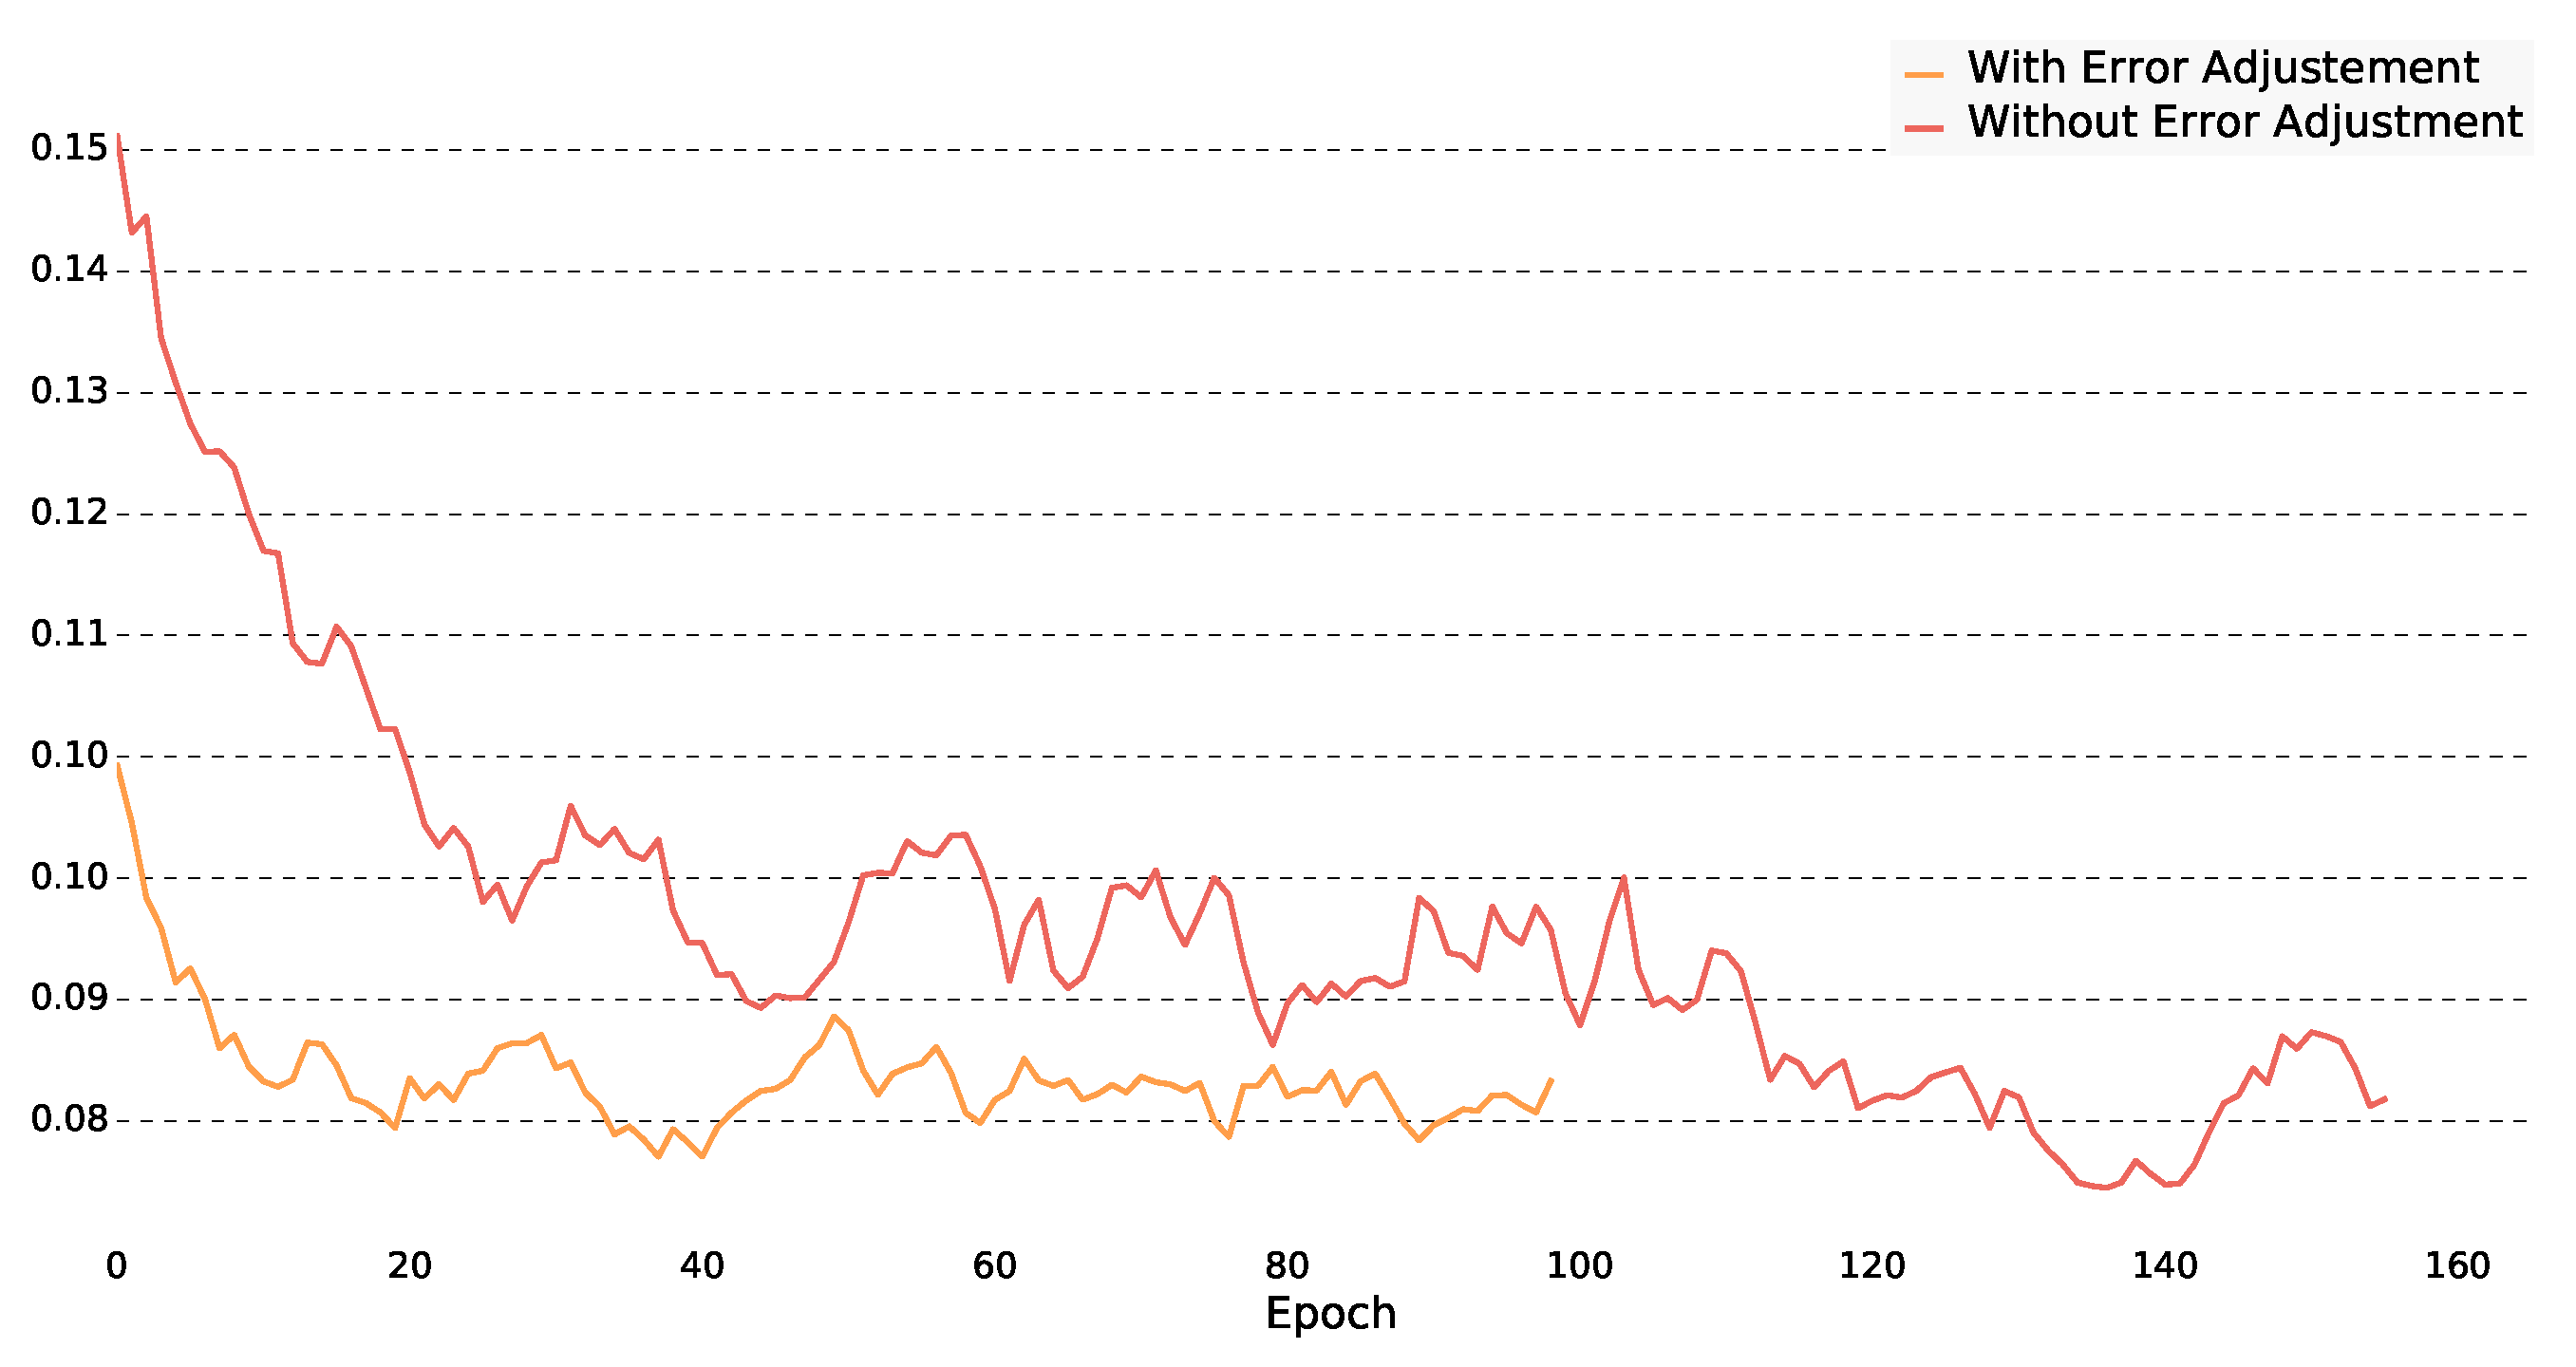
\includegraphics[width=\textwidth]{Graphics/cross_validation_fnn_unadj_vs_adj_error.eps}
\end{figure}
\end{frame}

\begin{frame}
\frametitle{Training}
  \justifying
\begin{figure}[h]
\centering
   Mean squared error on cross-validation set\\
   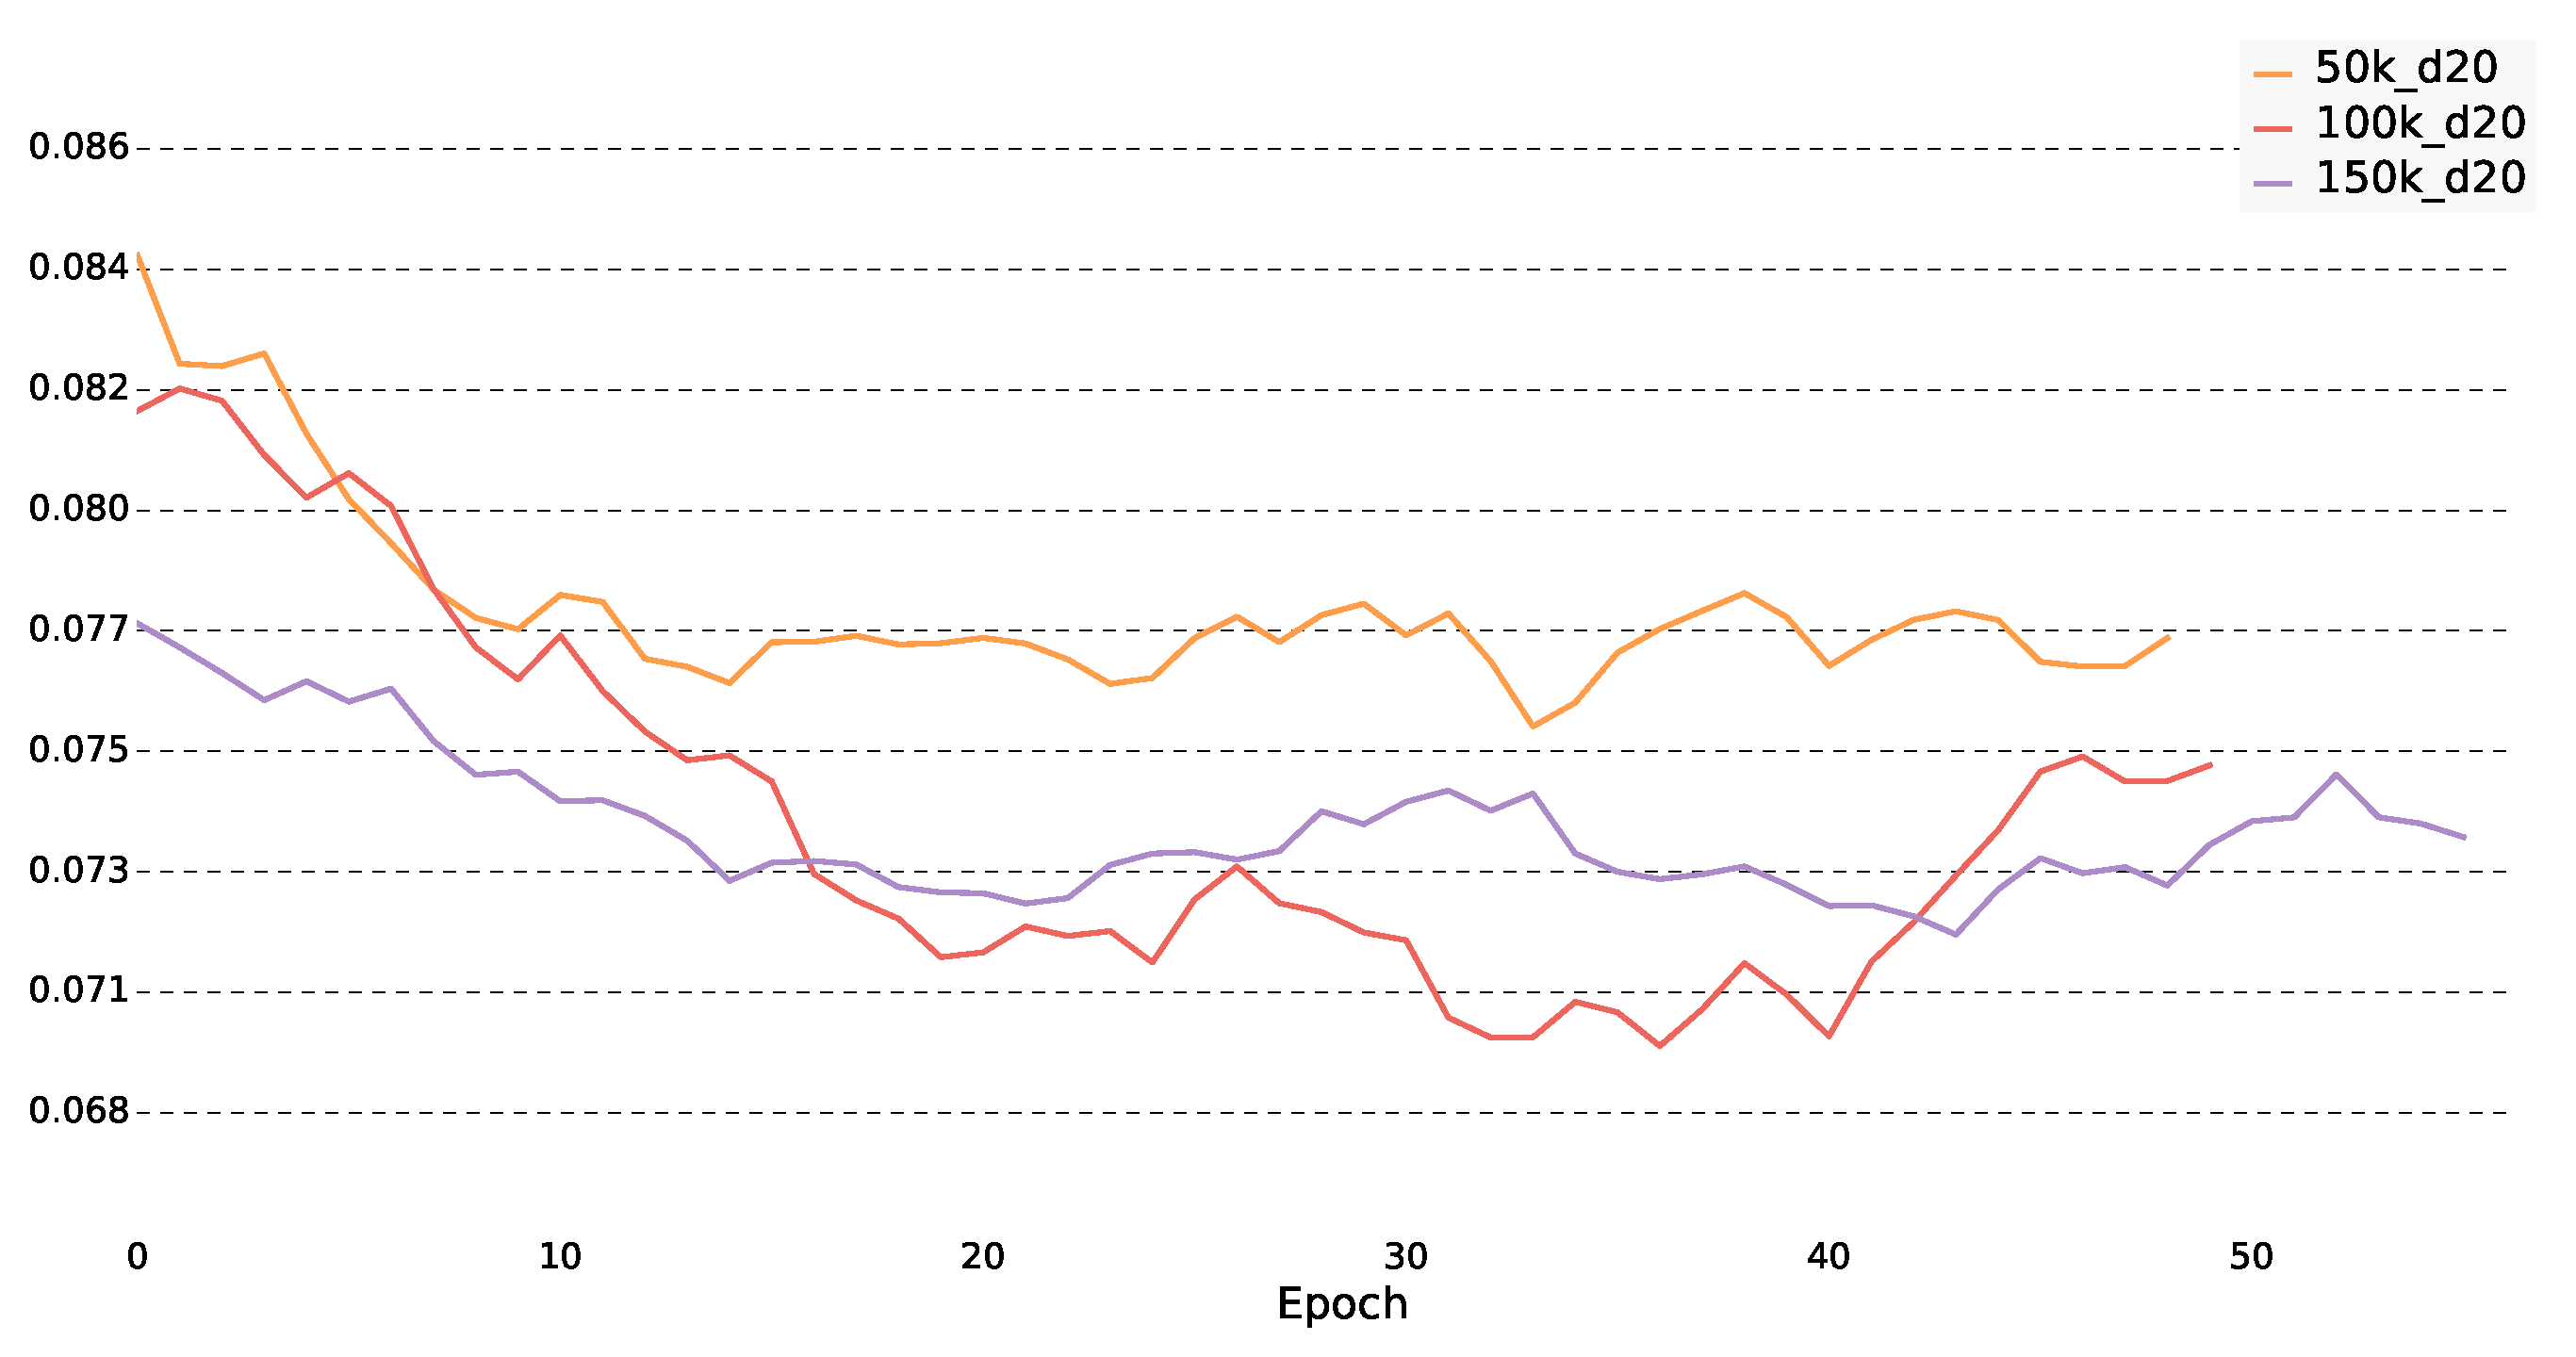
\includegraphics[width=\textwidth]{Graphics/adj_error_s_cross_validation_fnn.eps}
\end{figure}
\end{frame}


\subsection{Results}


\begin{frame}
\frametitle{Correlation from 01-2013 to 06-2014}
  \justifying
\begin{figure}[h]
\centering
   Average Volatily Error\\
   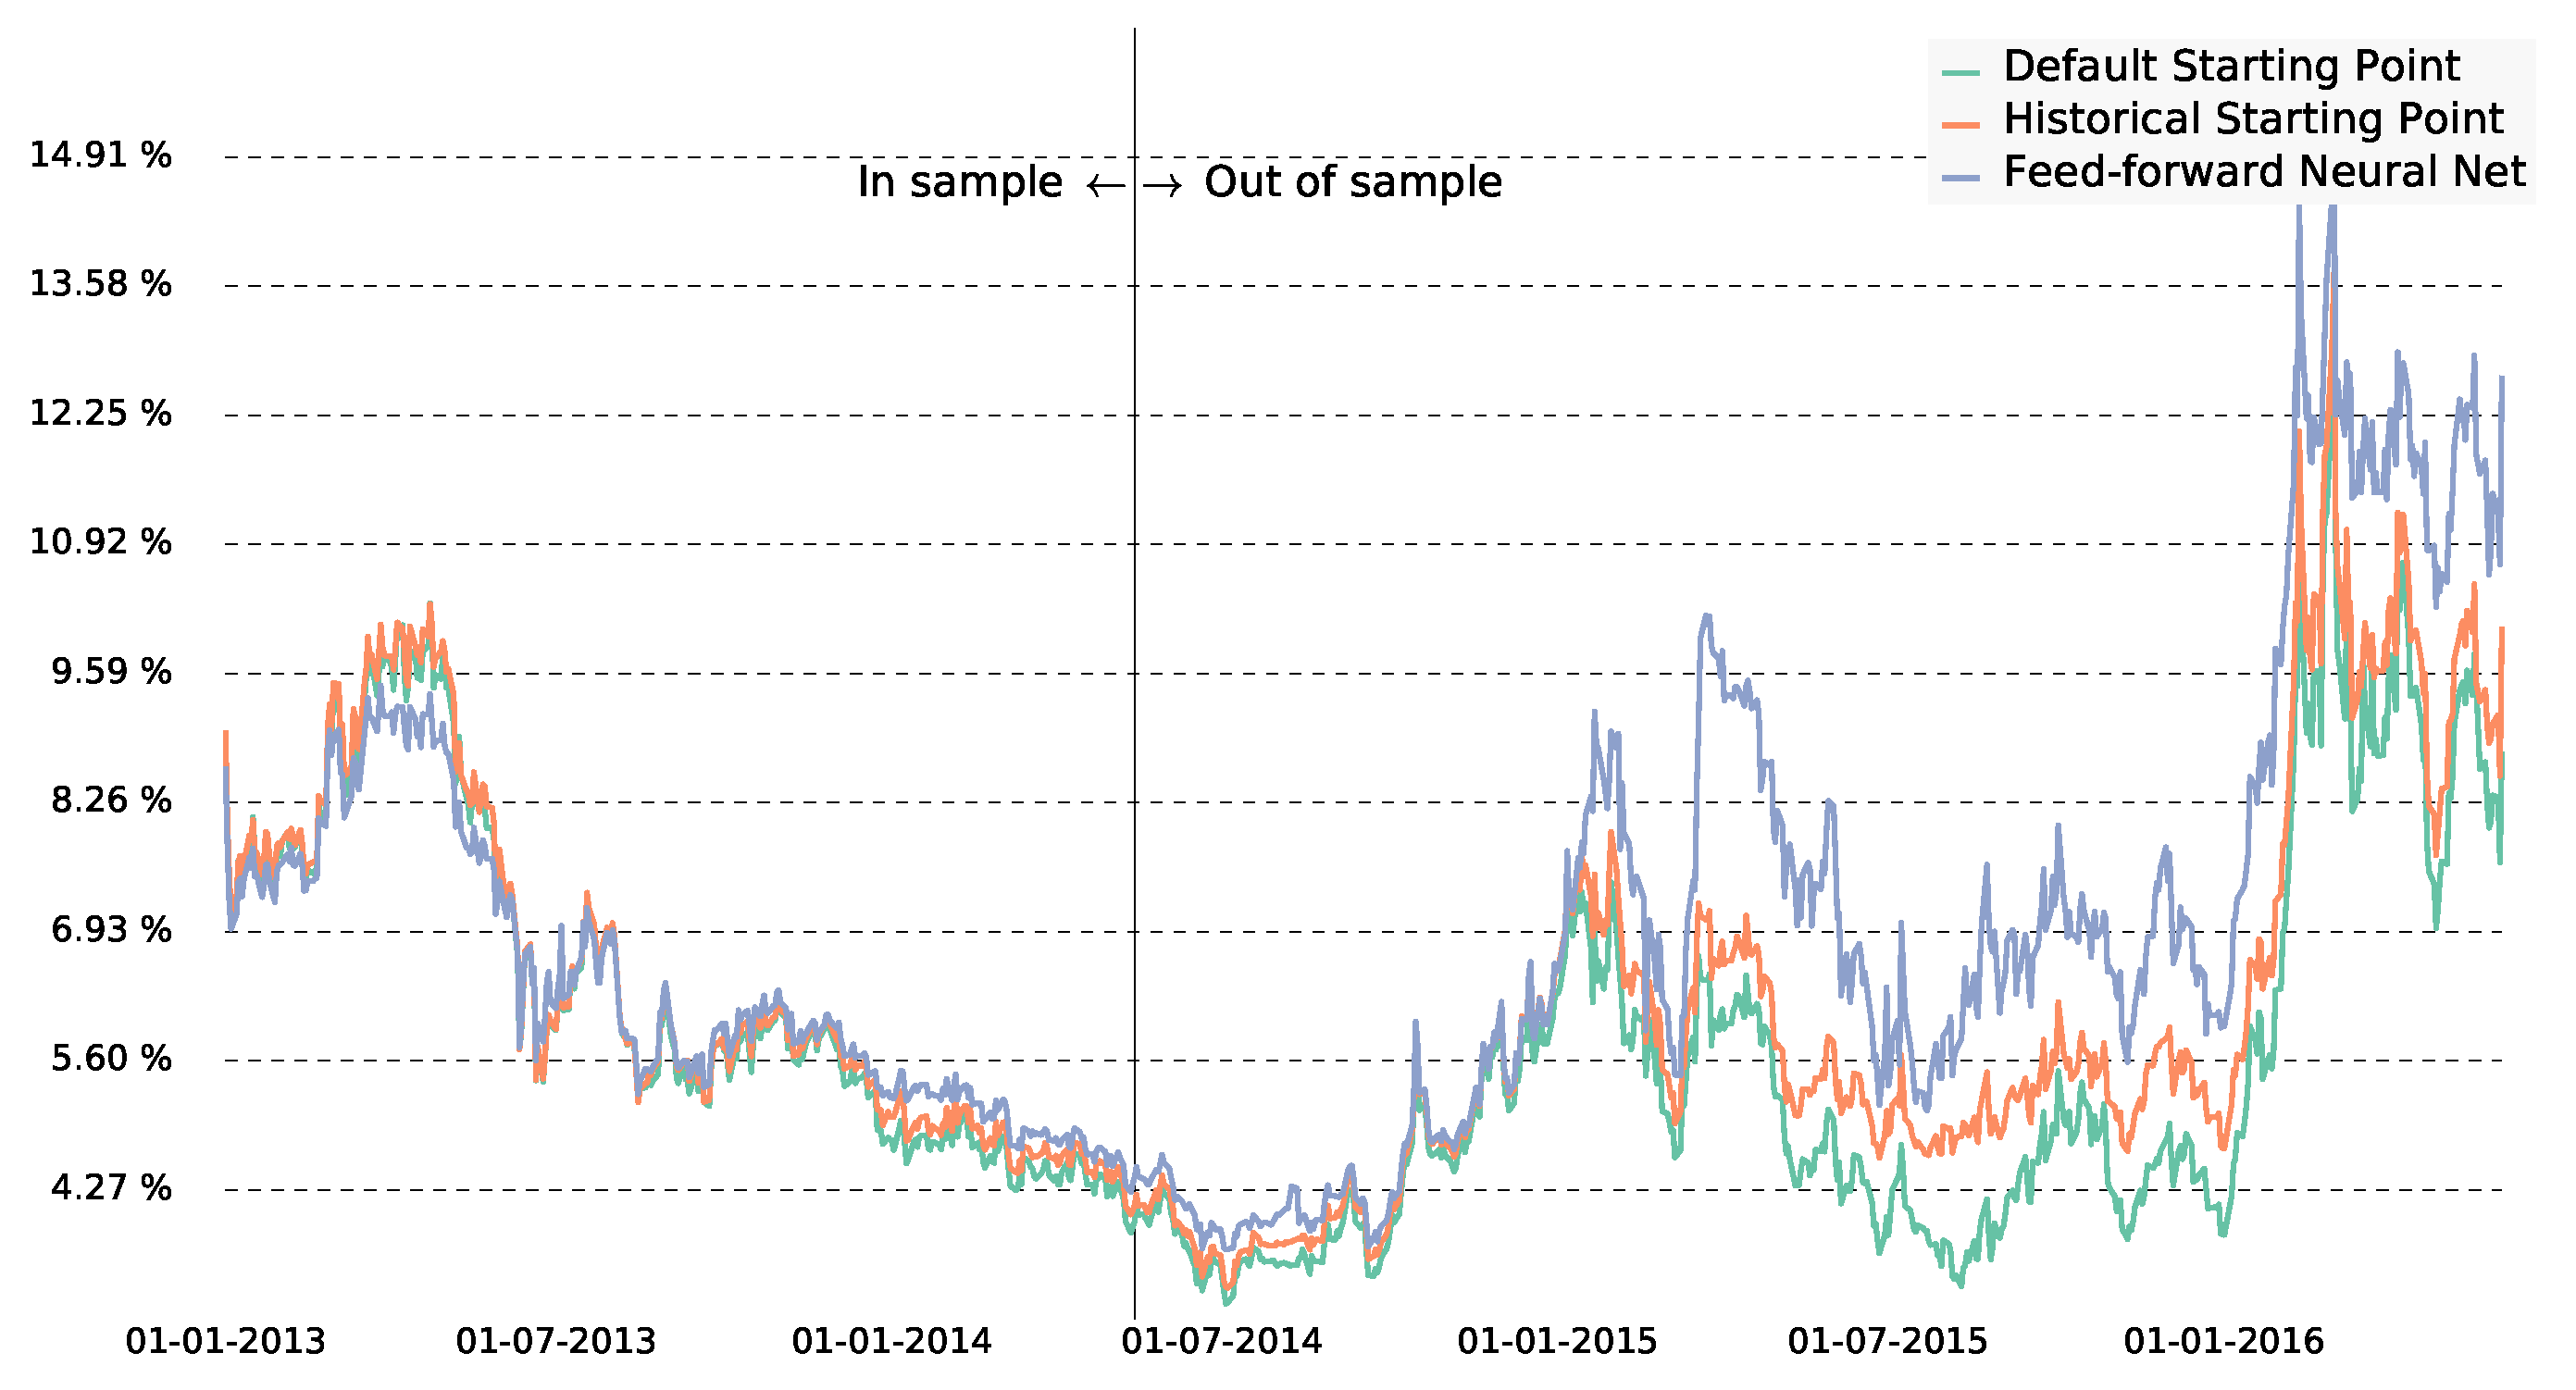
\includegraphics[width=\textwidth]{Graphics/adj_error_insample40_s150k_d20_vola_error_fnn.eps}
\end{figure}
\end{frame}

\begin{frame}
\frametitle{Correlation from 01-2013 to 06-2015}
  \justifying
\begin{figure}[h]
\centering
   Average Volatily Error\\
   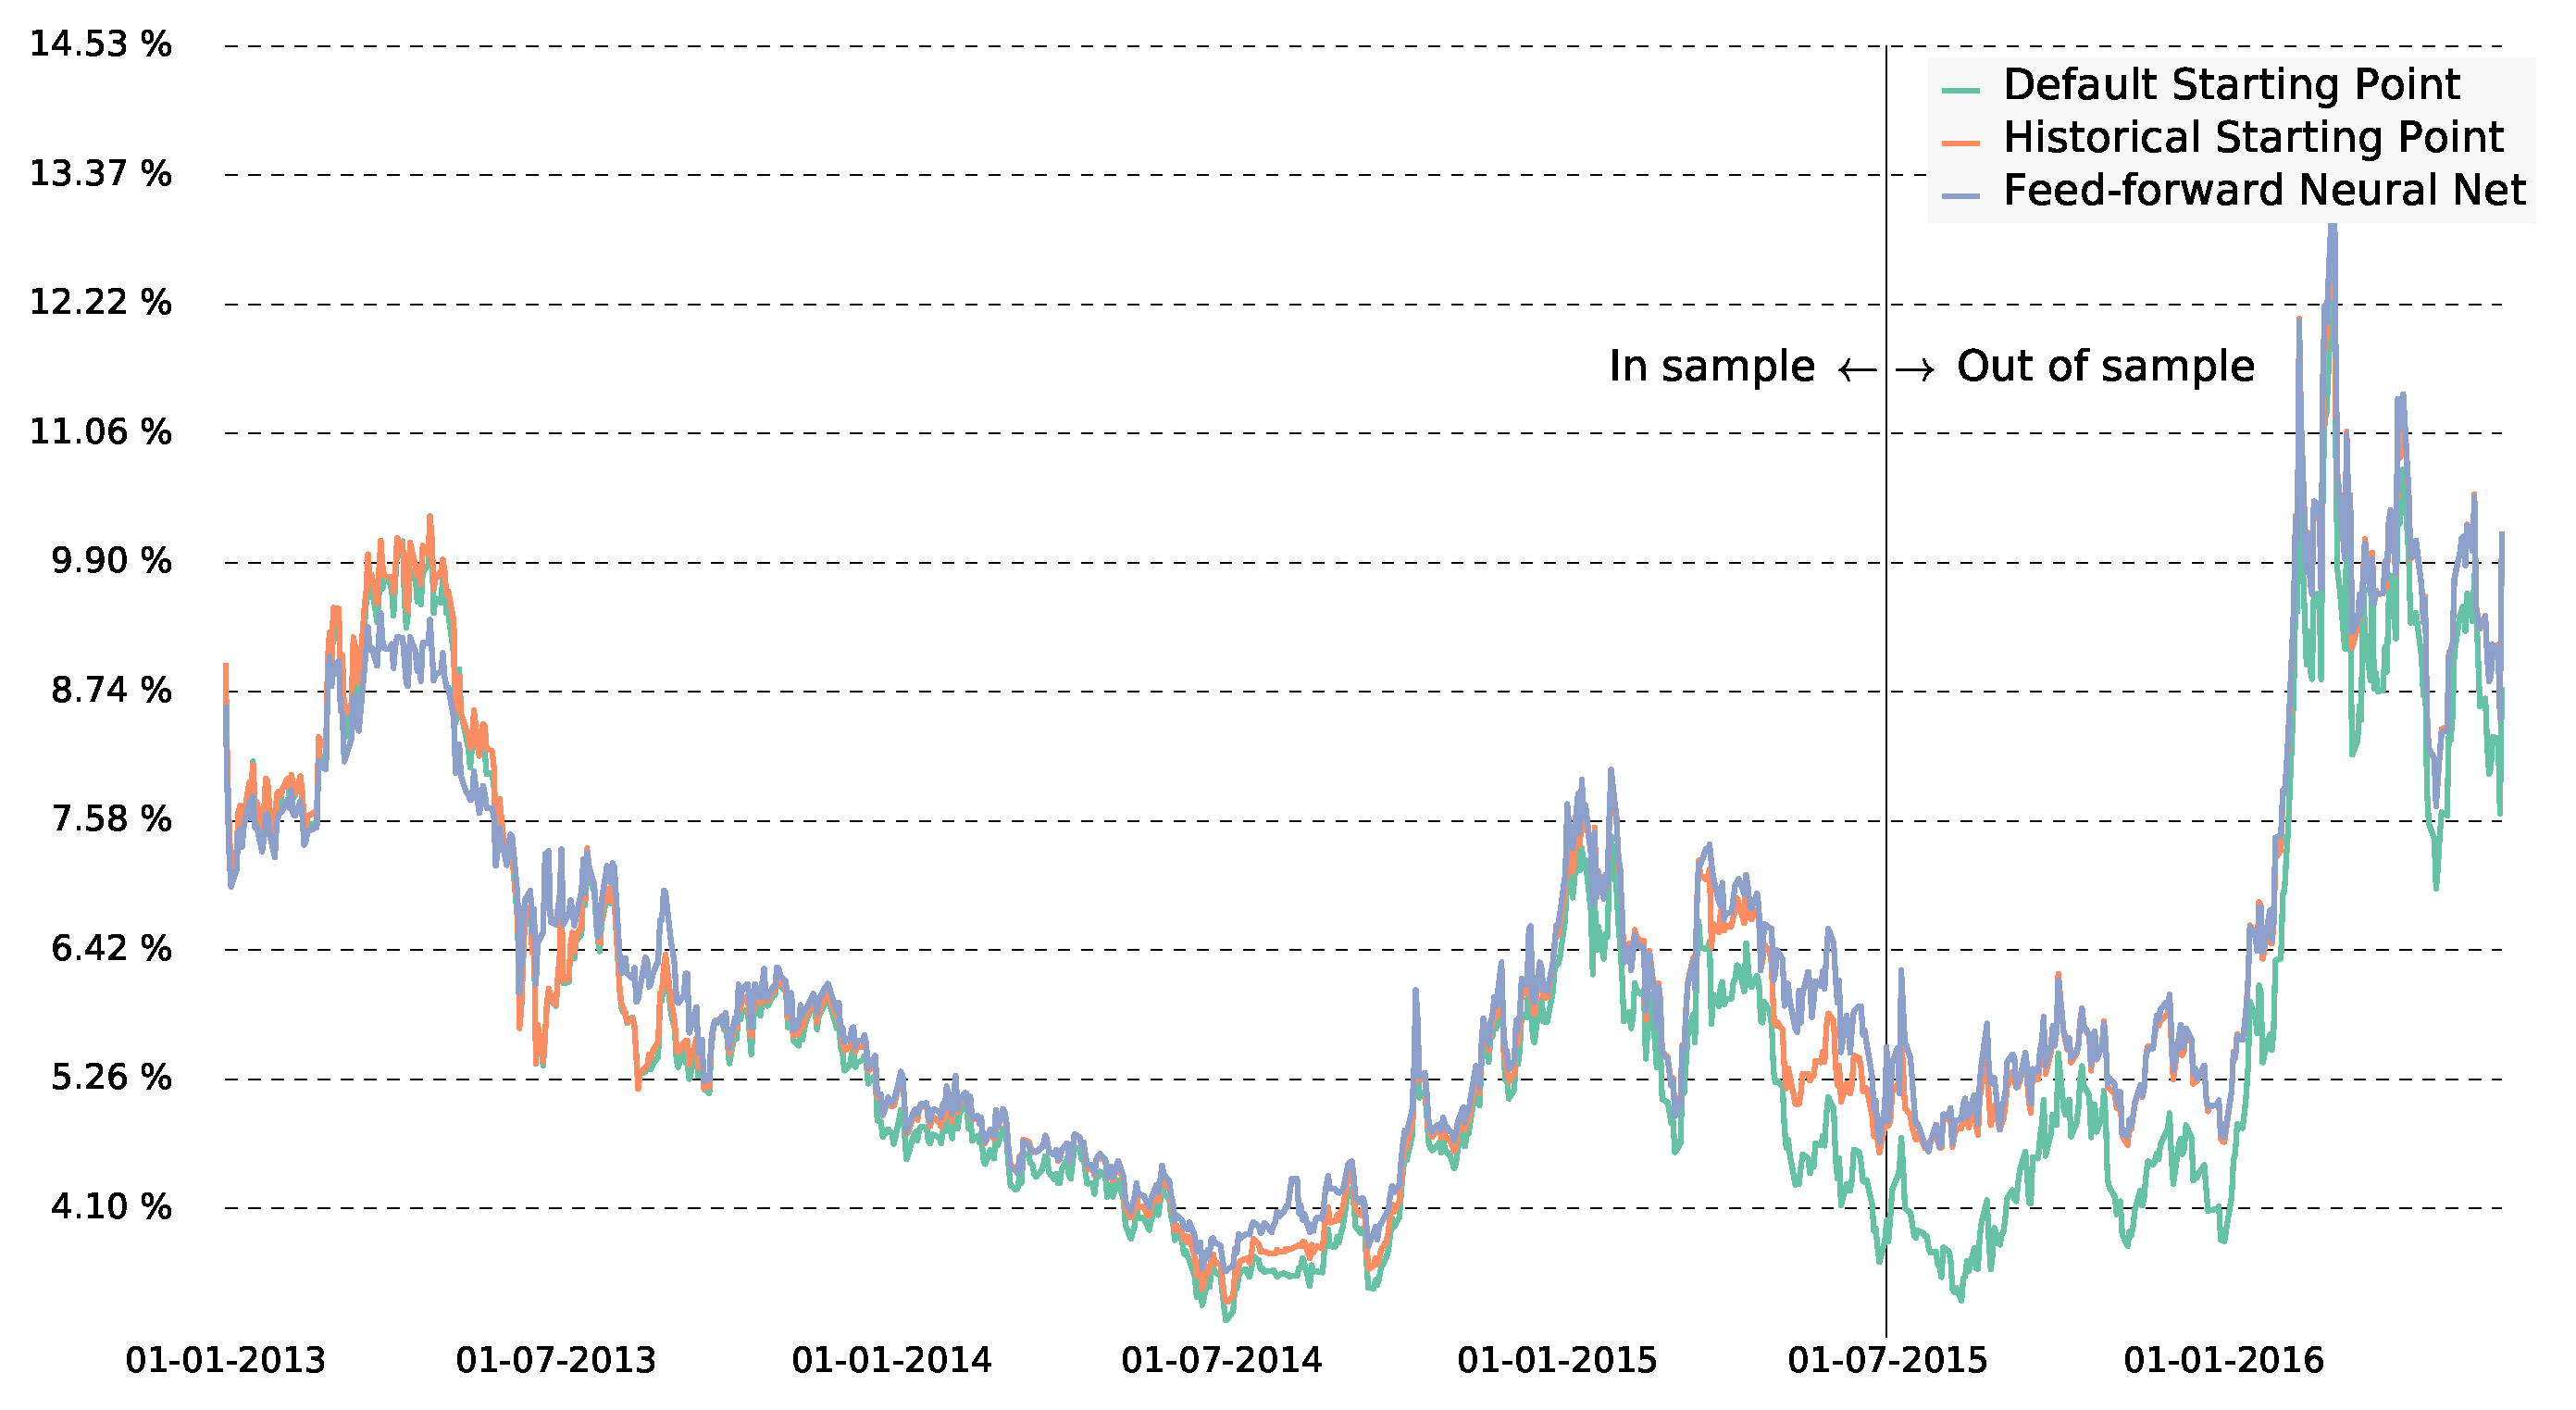
\includegraphics[width=\textwidth]{Graphics/adj_error_insample73_s150k_d20_vola_error_fnn.eps}
\end{figure}
\end{frame}

\begin{frame}
\frametitle{Correlation from 01-2013 to 06-2014}
  \justifying
\begin{figure}[h]
\centering
   Mean Square Error NPV\\
   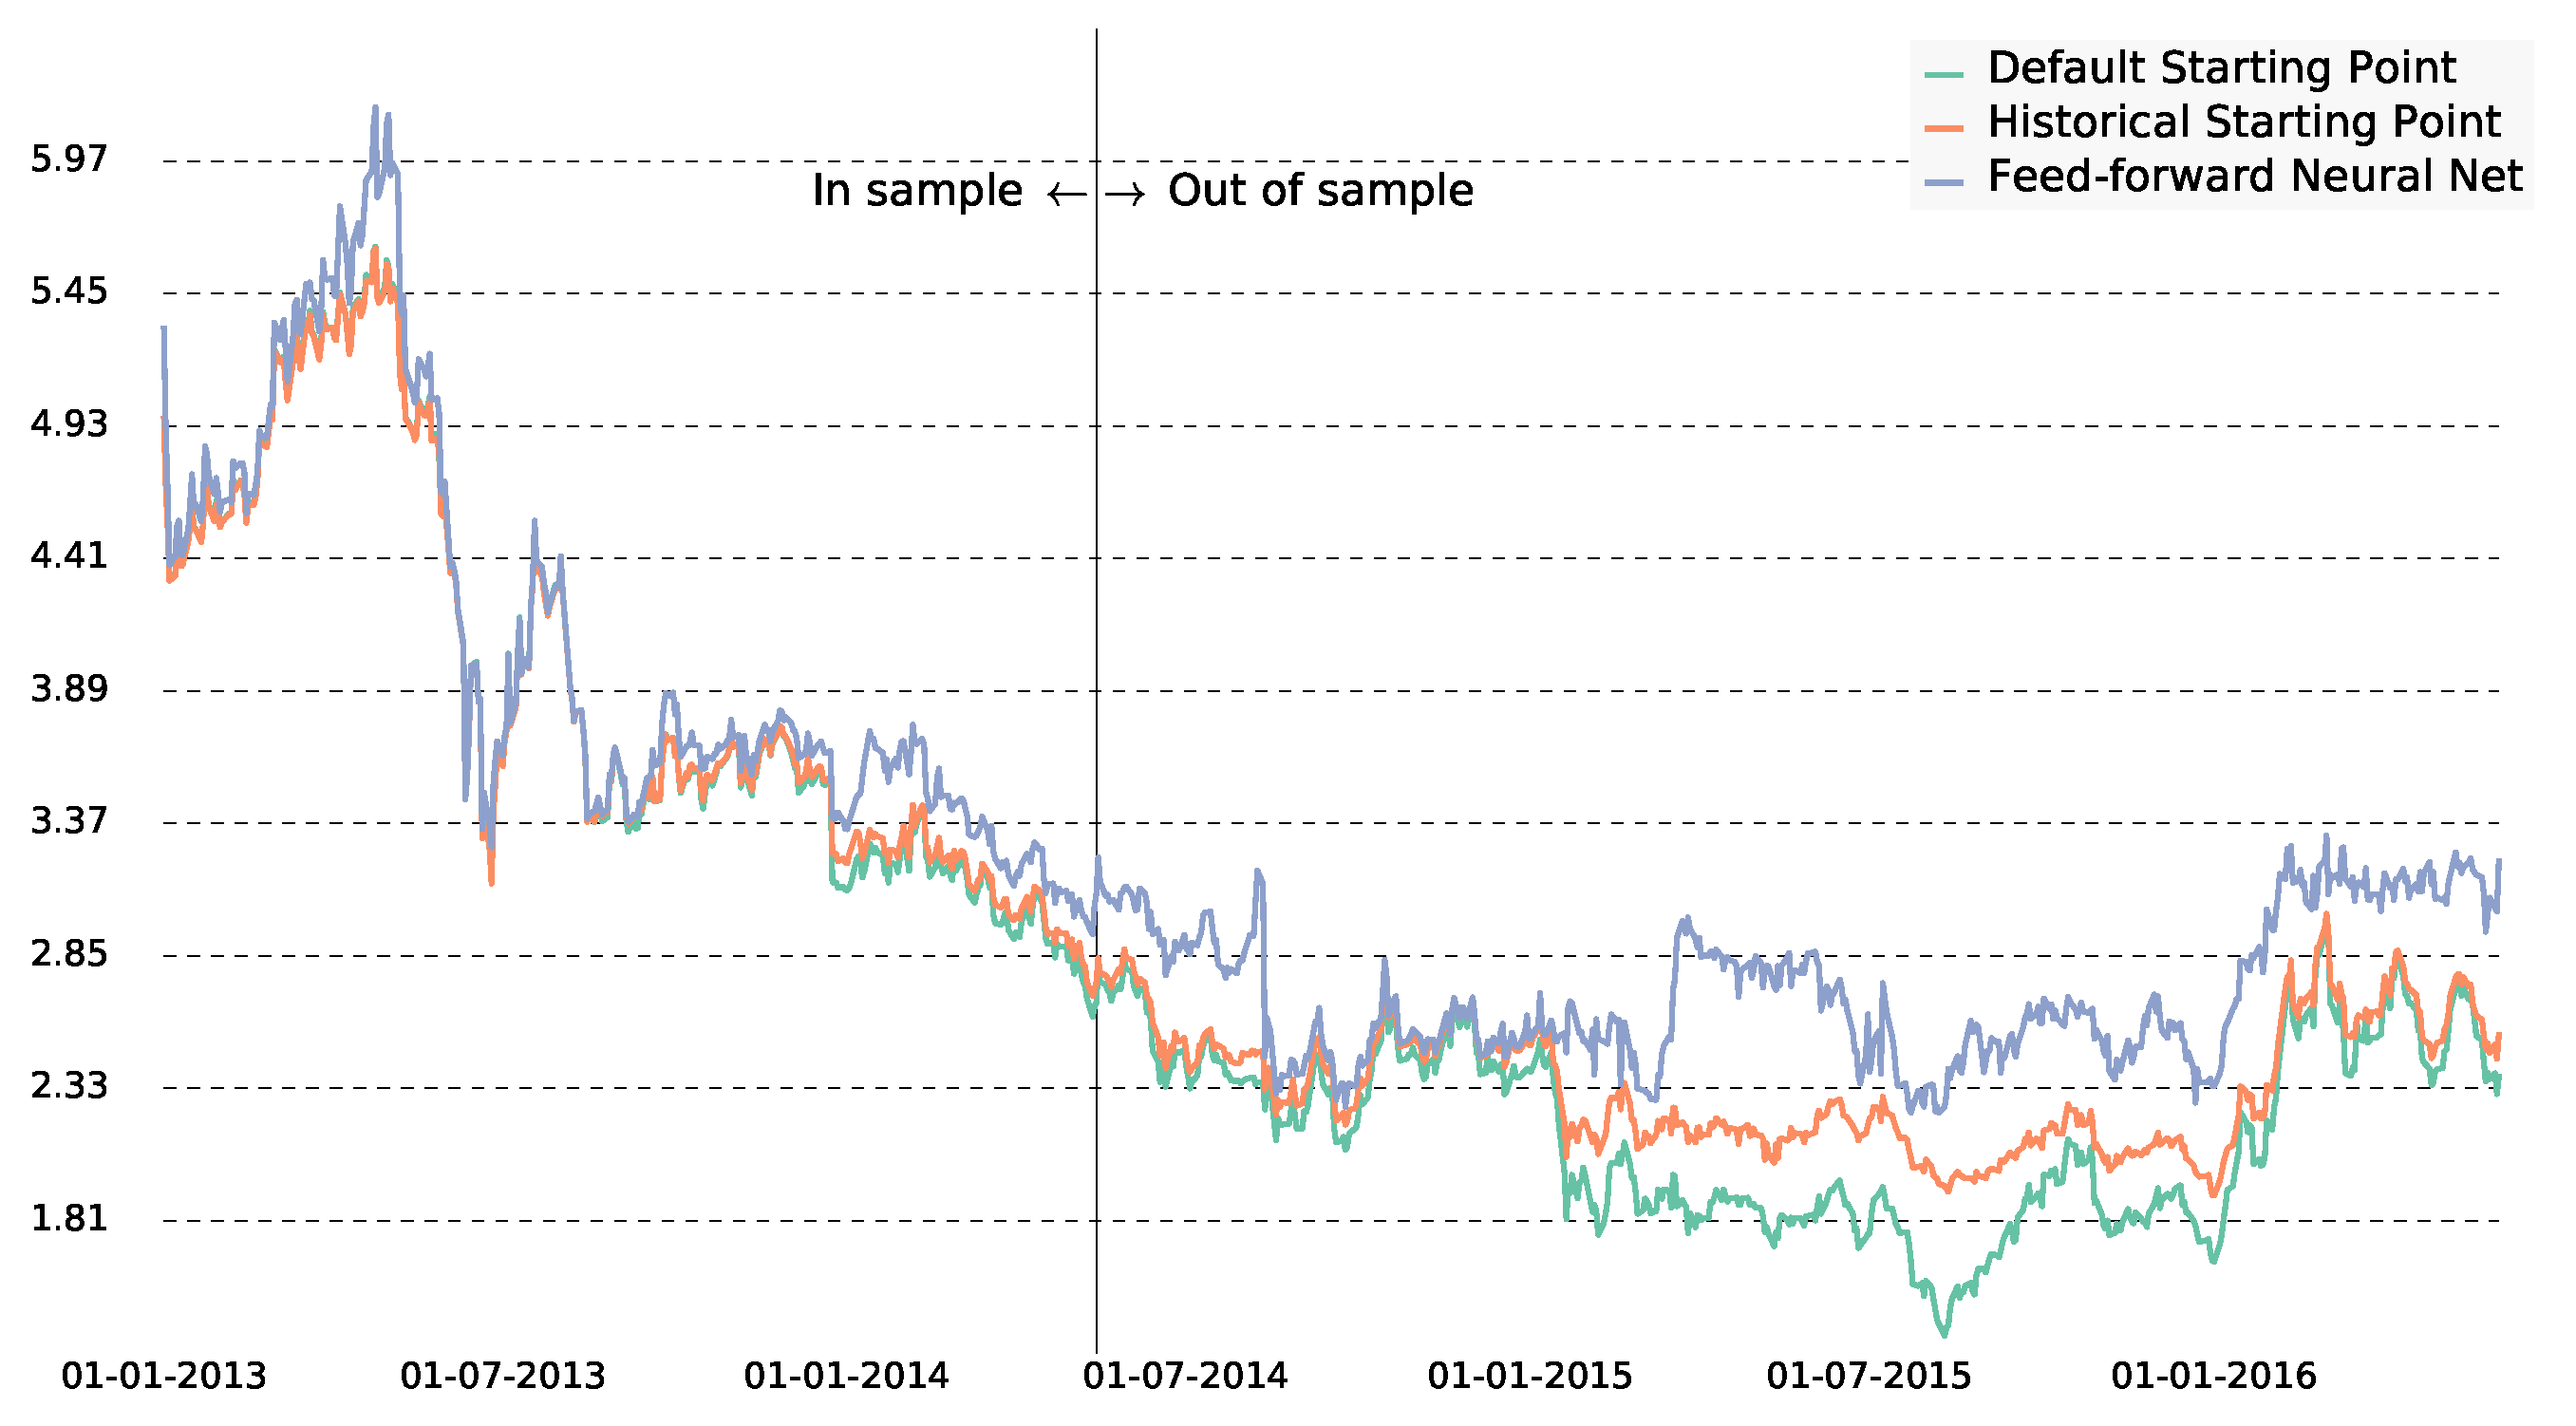
\includegraphics[width=\textwidth]{Graphics/adj_error_insample40_s150k_d20_npv_error_fnn.eps}
\end{figure}
\end{frame}

\begin{frame}
\frametitle{Correlation from 01-2013 to 06-2015}
  \justifying
\begin{figure}[h]
\centering
   Mean Square Error NPV\\
   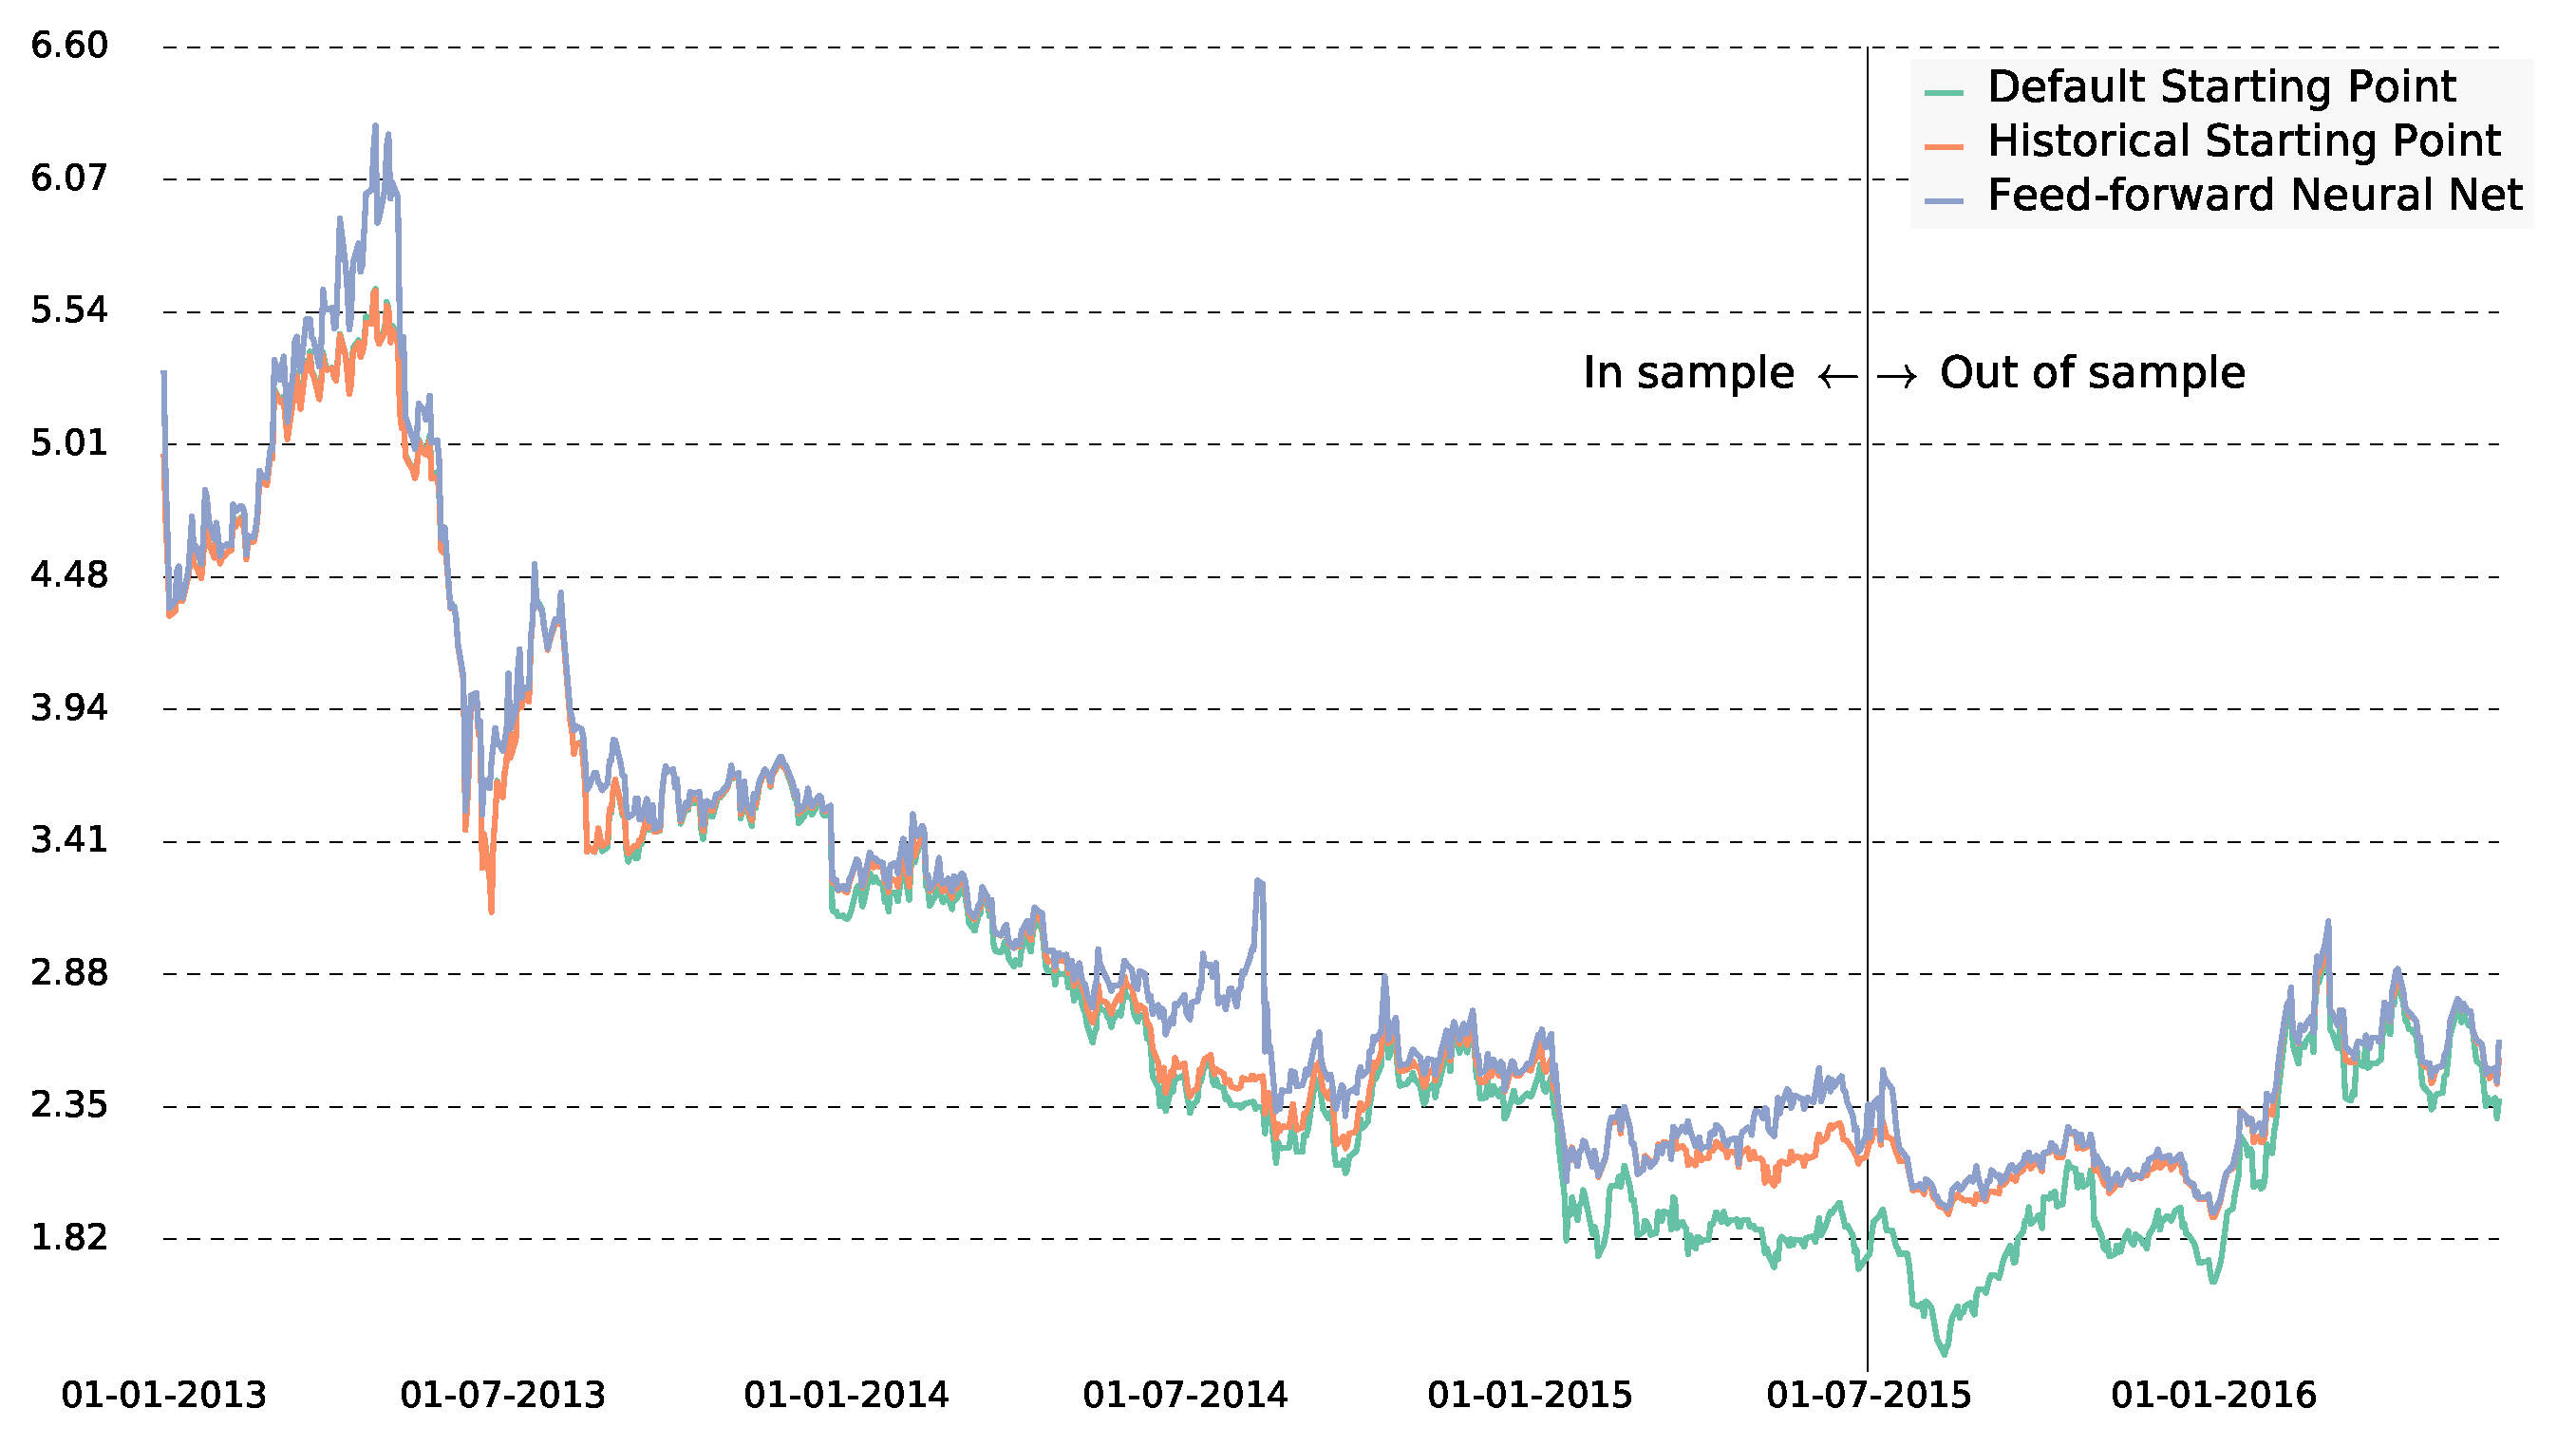
\includegraphics[width=\textwidth]{Graphics/adj_error_insample73_s150k_d20_npv_error_fnn.eps}
\end{figure}
\end{frame}

\begin{frame}
\frametitle{Cost Function on 01-07-2015}
  \justifying
 The historical point, lies on the trough. The default starting point ($\alpha=0.1$, $\sigma=0.01$) starts up on the side.
\begin{figure}[h]
\centering
    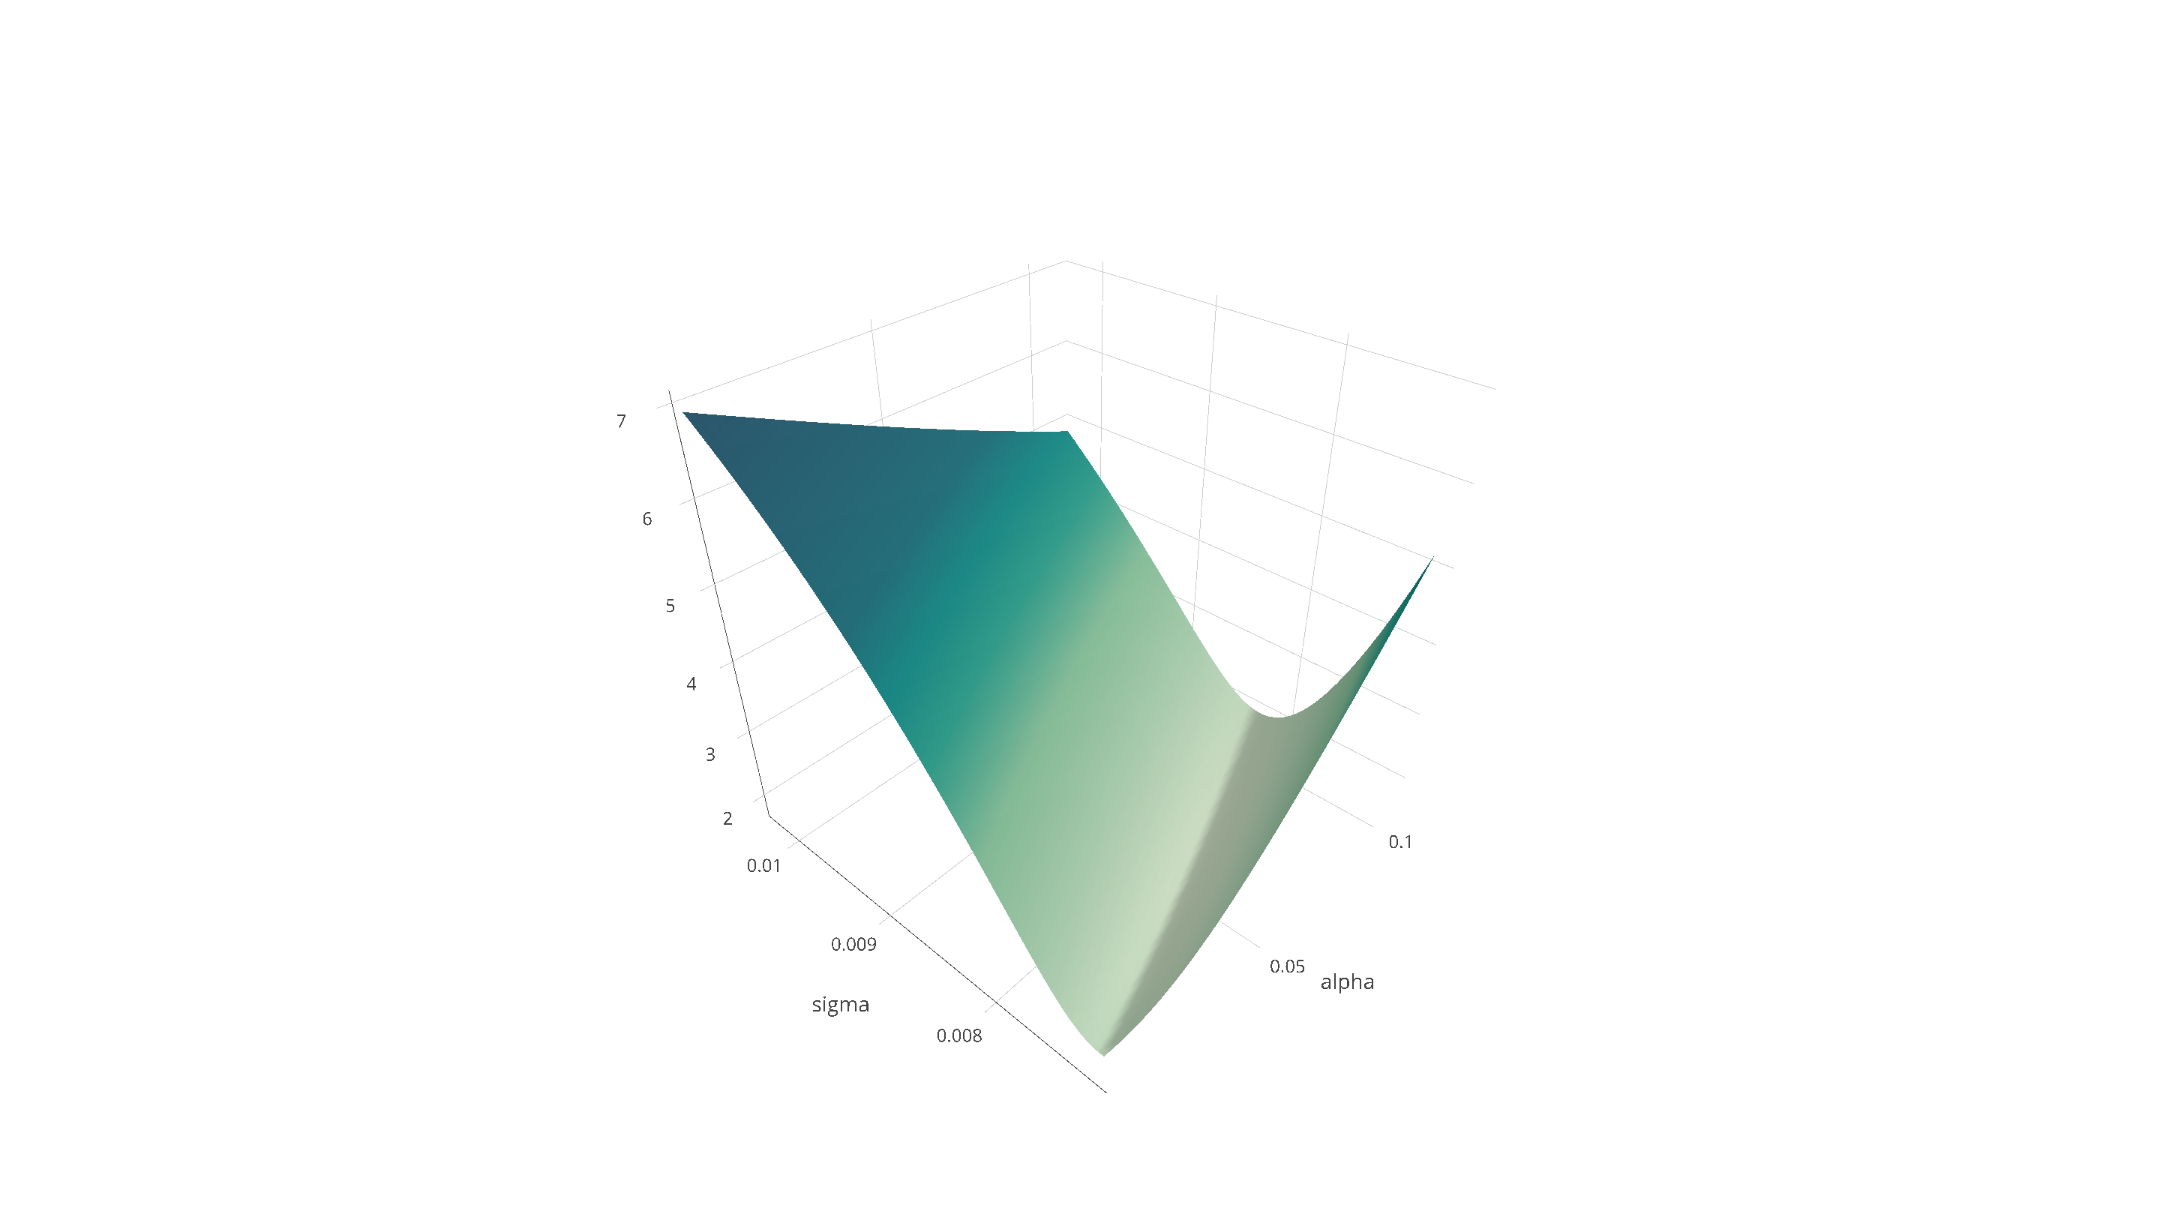
\includegraphics[width=\textwidth]{Graphics/surface.eps}
\end{figure}
\end{frame}

\begin{frame}
\frametitle{FNN}
  \justifying
\begin{figure}[h]
\centering
   Average Volatily Error\\
   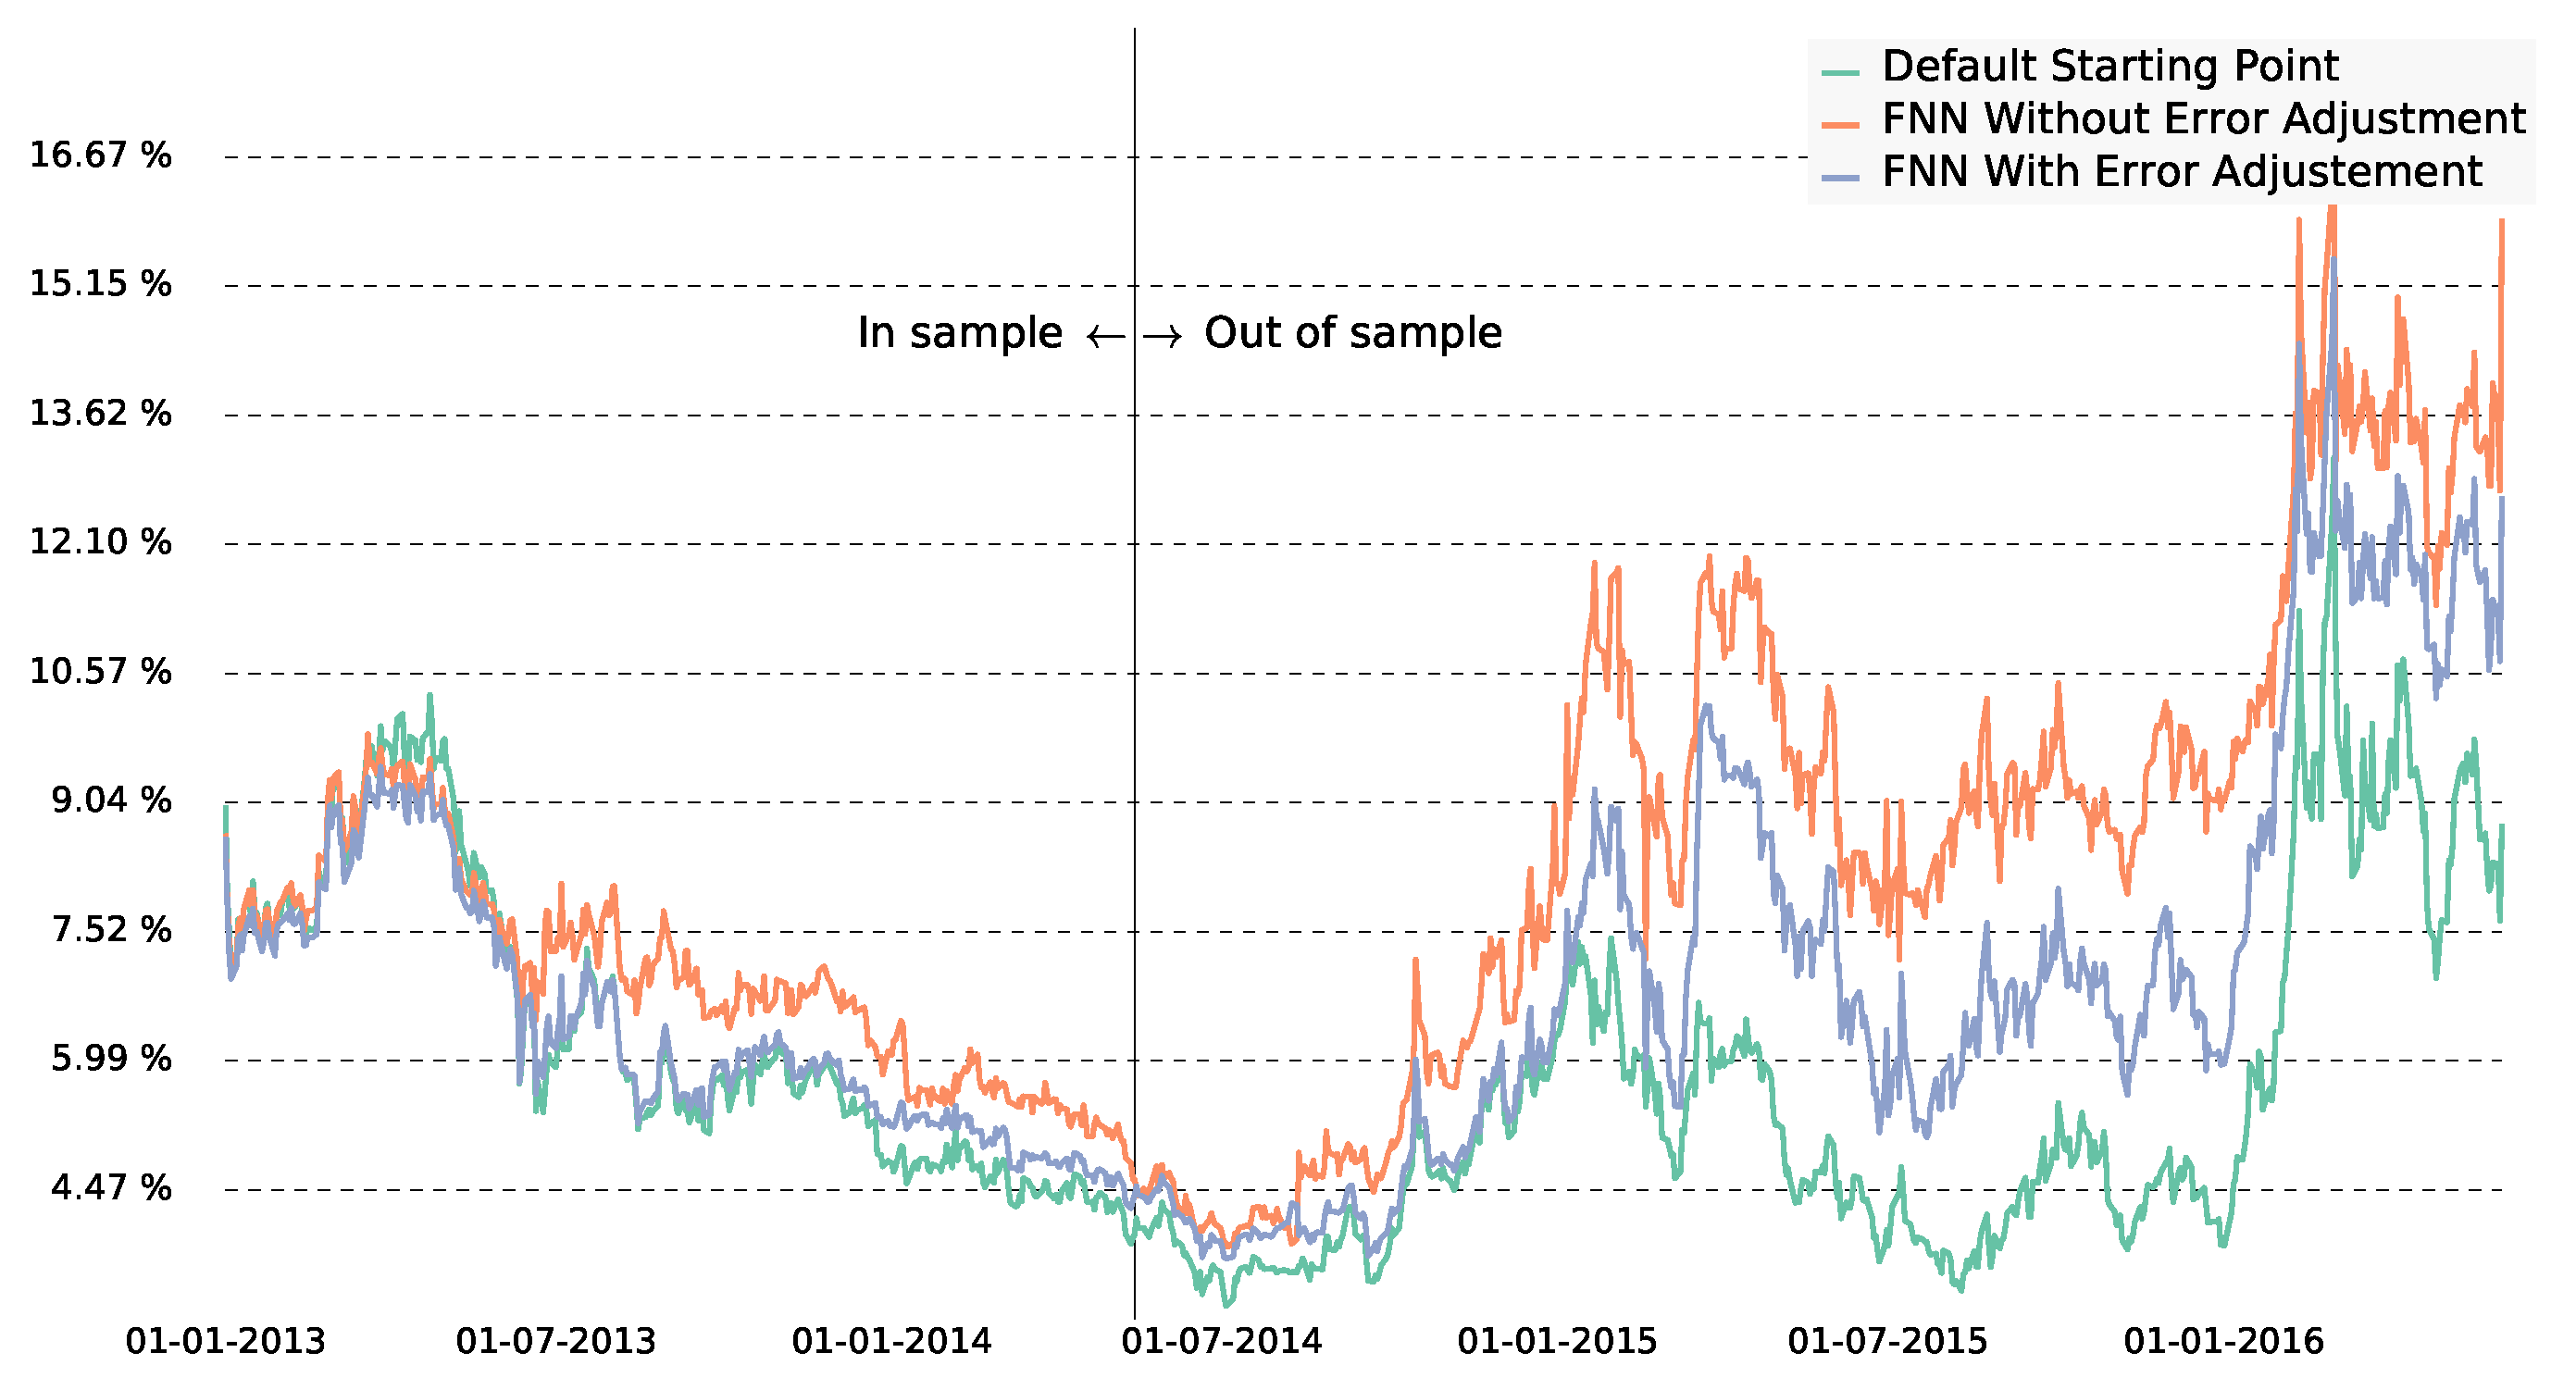
\includegraphics[width=\textwidth]{Graphics/vola_error_fnn_unadj_vs_adj_error.eps}
\end{figure}
\end{frame}

\begin{frame}
\frametitle{FNN}
  \justifying
\begin{figure}[h]
\centering
   Mean Square Error NPV\\
   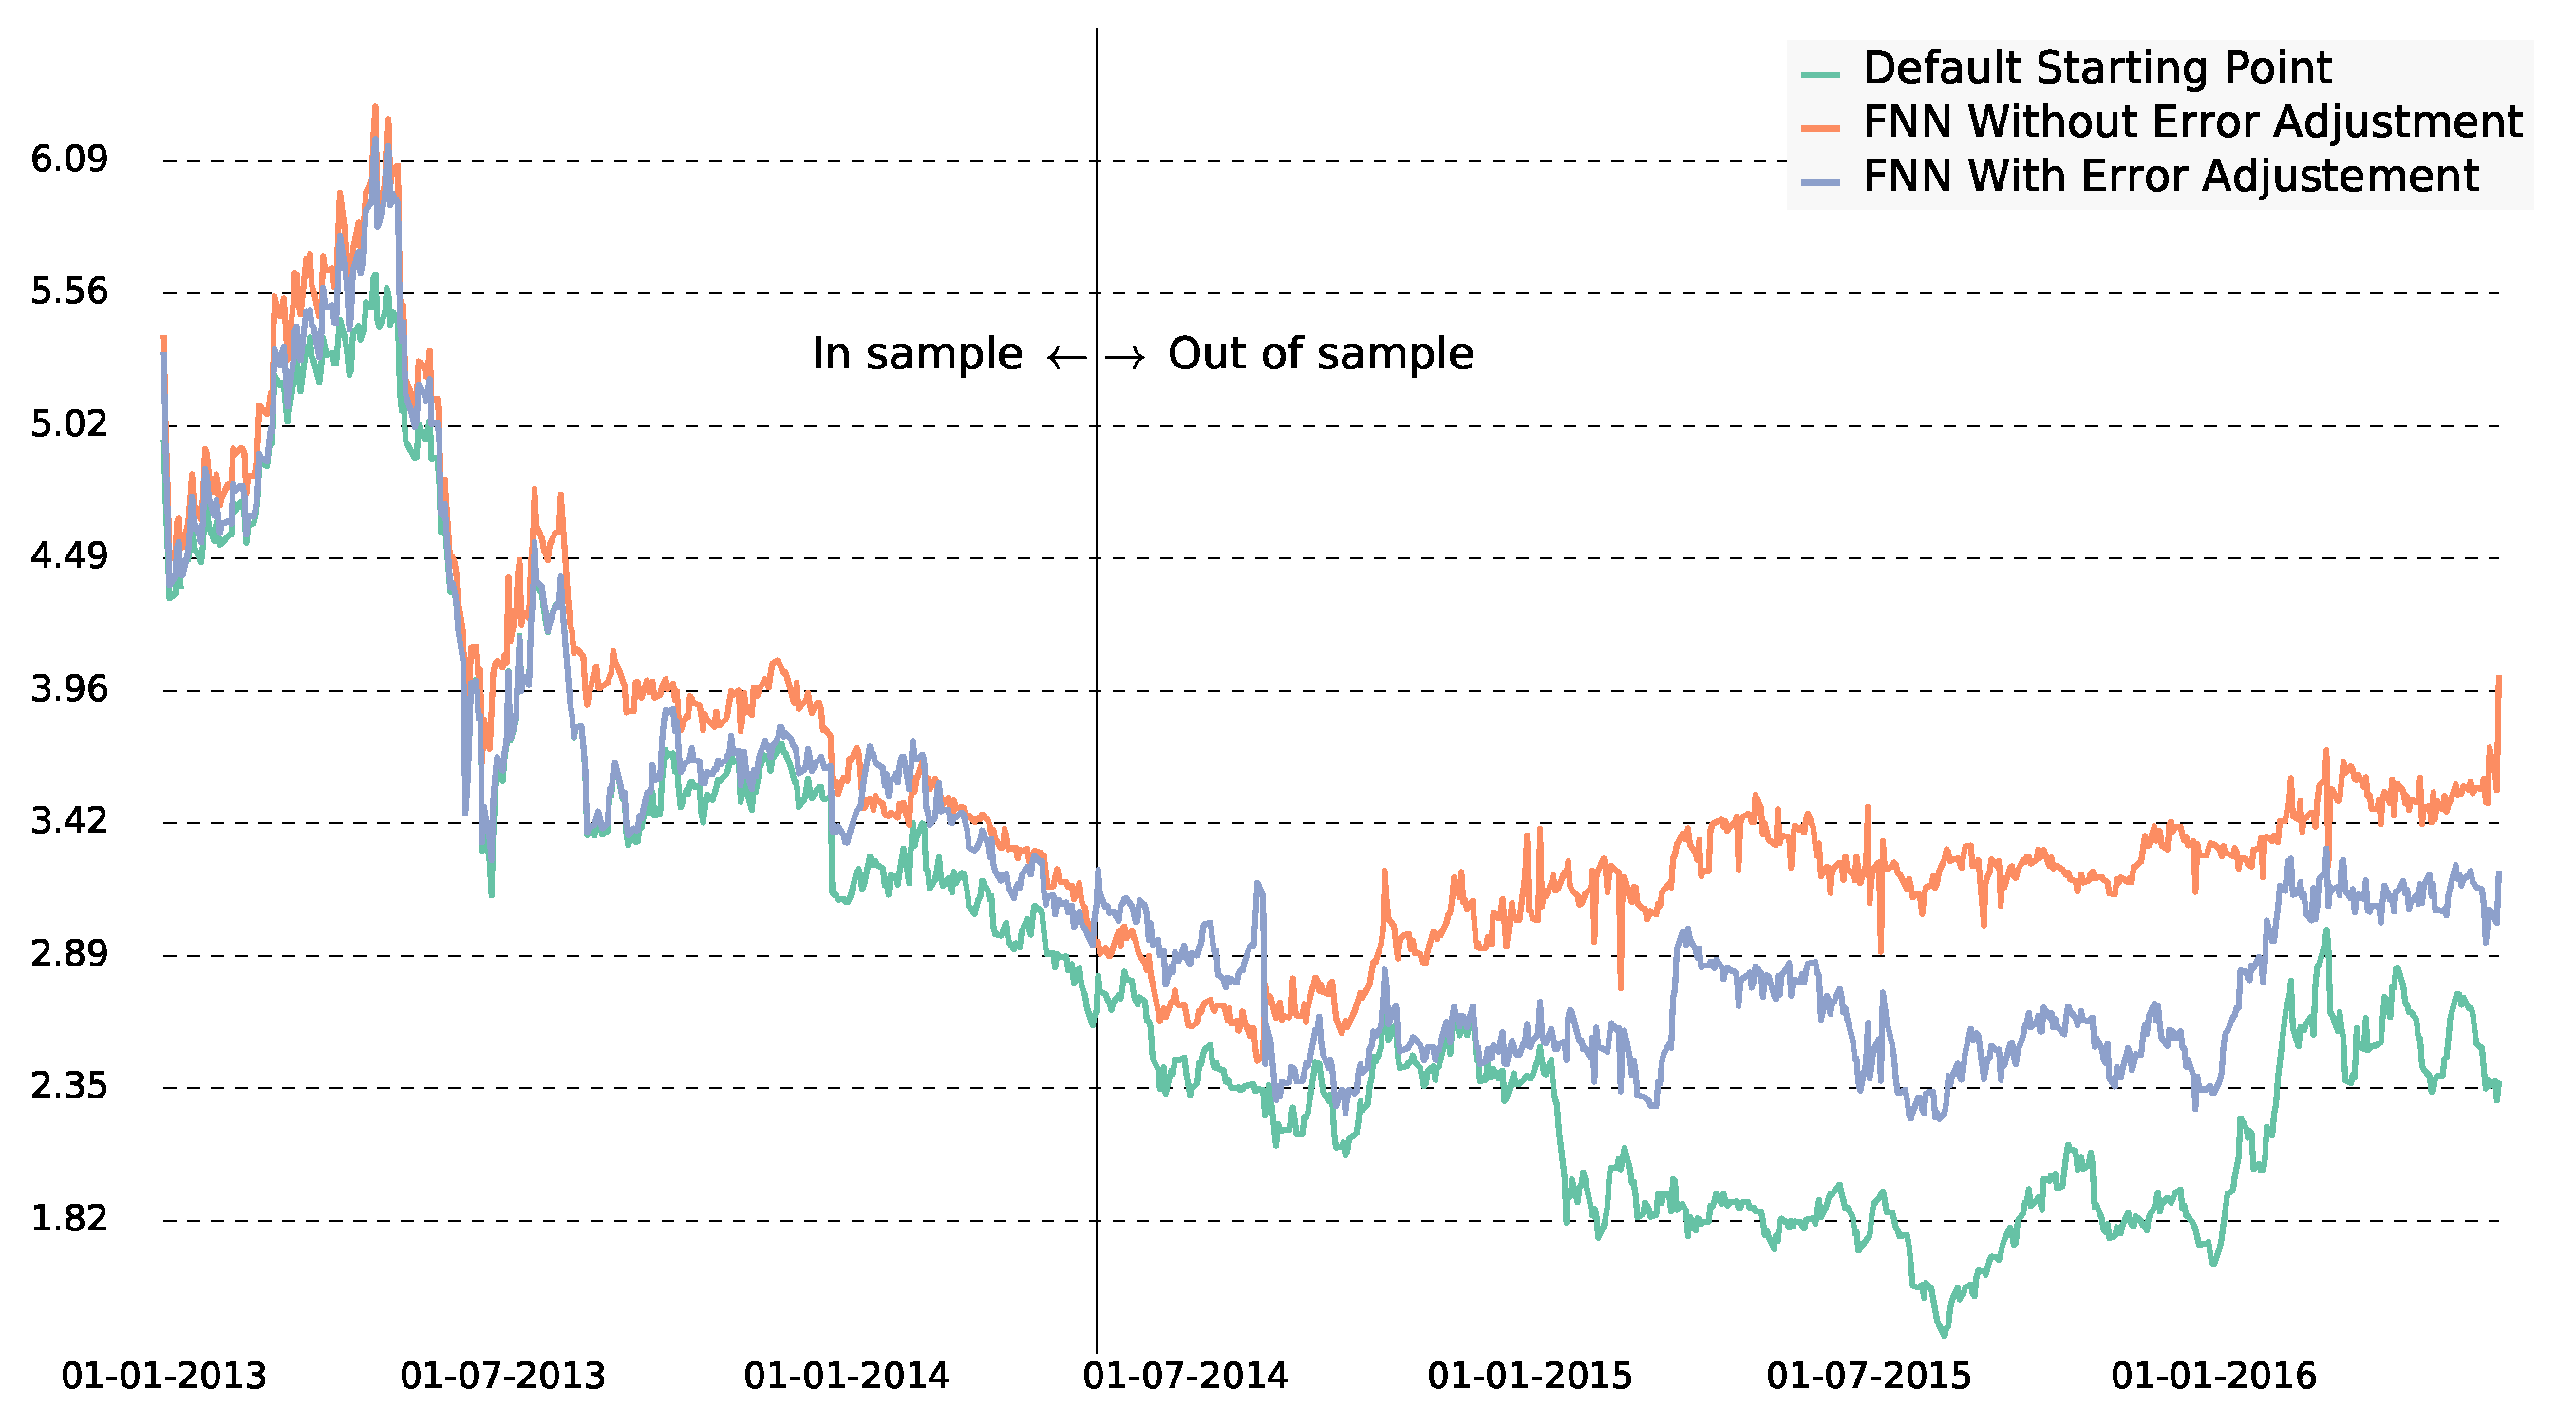
\includegraphics[width=\textwidth]{Graphics/npv_error_fnn_unadj_vs_adj_error.eps}
\end{figure}
\end{frame}

\begin{frame}
\frametitle{Further work}
  \justifying

\begin{itemize}
\item Sample with parameterized correlation
\item Test with equity volatility models. In particular with large volatility surface and use convolutional neural networks
\item Test with more complex IR models
\end{itemize}
\end{frame}

\begin{frame}
\frametitle{Accessing it}
  \justifying
The example detailed here can be found in my GitHub account:
\url{https://github.com/Andres-Hernandez/CalibrationNN}

To run the code, the following python packages are needed:
\begin{itemize}
\item QuantLib
\item QuantLib Python SWIG bindings
\item Typical python numerical packages: numpy, scipy, pandas, sklearn (, matplotlib)
\item \href{http://keras.io/}{Keras}: a deep-learning python library. Requires Theano or TensorFlow as backend
\end{itemize}
\end{frame}
\end{document}
